\chapter{Schémas aux différences}

\section{Opérateurs aux différences en dimension 1}

\subsection{Notations}
\label{sec:notation_1D}

On considère $\Omega = [a,b]$, $a<b$, un intervalle de $\mathbb{R}$ de longueur $L=b-a$. Nous utilisons les lettres latines pour noter les fonctions continues : $f(x)$, $u(x)$, ... $x \in \Omega$. Pour $u$ et $v$, des fonctions définies sur $\Omega$, le produit scalaire dans $L^2 ( \Omega )$ est défini par
\begin{equation}
(u,v) = \gint_{\Omega} u(x) \bar{v}(x) dx = \gint_{a}^b u(x) \bar{v}(x) dx.
\end{equation}
Pour $u$ et $v$ à valeurs réelles, on a
\begin{equation}
(u,v) = \gint_{a}^b u(x) v(x) dx.
\end{equation}
La norme sur $L^2(\Omega)$ est donnée par :
\begin{equation}
\| u \|_{L^2(\Omega)} = \sqrt{(u,u)}
\end{equation}
Pour $u \in L^{\infty}(\Omega)$, on note
\begin{equation}
\| u \|_{\infty} = \sup_{x\in\Omega} |u(x)|.
\end{equation}
Une fonction $u : x \in \mathbb{R} \mapsto u(x) \in \mathbb{R}$ est \textit{périodique} de période $L$ si 
\begin{equation}
u(x+L) = u(x) \text{, } \forall x \in \mathbb{R}.
\end{equation}
En particulier, on a $u(a)=u(b)$.

On considère une grille régulière sur $\Omega$ constituée de $N \geq 1$ points :
\begin{equation}
a=x_0 < x_1 < \ldots < x_{N-1} < x_N = b,
\end{equation}
où les valeurs $x_i$ sont définies par :
\begin{equation}
x_i = a + ih\text{, } i = 0,1, \ldots,N \text{ et } h = \dfrac{b-a}{N} \text{ le pas d'espace}. 
\end{equation}

\begin{figure}[htbp]
\begin{center}
\begin{tikzpicture}[scale=1.8]
	\draw [>=stealth, <->] (-2,0.2) -- (-1,.2) ;
	\draw (-1.5,.3) node[above] {$h$} ;
	\draw (-3,0) -- (3,0) ;
	\draw (-3,0) node {$\times$} ;
	\draw (-3,-.2) node[below] {$x_0=a$} ;
	\draw (-2,0) node {$\bullet$} ;
	\draw (-2,-.2) node[below] {$x_1$} ;
	\draw (-1,0) node {$\bullet$} ;
	\draw (-1,-.2) node[below] {$x_2$} ;
	\draw (0,-.2) node[below] {$\ldots$} ;
	\draw (1,0) node {$\bullet$} ;
	\draw (1,-.2) node[below] {$x_{N-2}$} ;
	\draw (2,0) node {$\bullet$} ;
	\draw (2,-.2) node[below] {$x_{N-1}$} ;
	\draw (3,0) node {$\times$} ;
	\draw (3,-.2) node[below] {$x_N =b$} ;
\end{tikzpicture}
\end{center}
\caption{Grille en dimension 1. Les symboles $\times$ désignent les points de bords, les symboles $\bullet$ désignent les points intérieurs de la grille.}
\label{fig:maillage1D}
\end{figure}

Les points $x_0=a$ et $x_N = a + L = b$ sont les points de bord du domaine et les points $(x_j)_{1 \leq j \leq N-1}$ désignent les points intérieurs. 

Nous distinguons trois types de données aux points de grille $x_j$, $0 \leq j \leq N$ :
\begin{enumerate}
\item Une \textit{fonction de grille} est une fonction définie uniquement aux points $(x_j)_{0 \leq j \leq N}$. Les fonctions de grilles sont notées en fonte gothique : $\mathfrak{u}$, $\mathfrak{v}$, ... 
On note
\begin{equation}
\mathfrak{u} = (\mathfrak{u}(x_0), \mathfrak{u}(x_1), \mathfrak{u}(x_2), ... , \mathfrak{u}(x_N)).
\end{equation}
De plus, $l^2_h$ désigne l'espace des fonctions de grille, $h>0$ fixé.
On munit cet espace du produit scalaire et de la norme associée :
\begin{equation}
(\mathfrak{u},\mathfrak{v})_h = h \gsum_{j=0}^N \mathfrak{u}(x_j) \mathfrak{v}(x_j) \text{,  } |\mathfrak{u}|_h^2 = h \gsum_{j=0}^N \mathfrak{u}(x_j)^2.
\end{equation}
On définit aussi la norme infinie pour les fonctions de grille :
\begin{equation}
\| \mathfrak{u} \|_{\infty} = \max_{0\leq j \leq N} |\mathfrak{u}(x_j)|.
\end{equation}
On notera 
\begin{equation}
\mathfrak{u}_j = \mathfrak{u}(x_j) \text{ pour tout } 0\leq j \leq N.  
\end{equation}

On note $l^2_{h,per}$ l'espace des fonctions de grilles périodiques. Si $\mathfrak{u} \in l^2_{h,per}$ alors $\mathfrak{u}(x_0) = \mathfrak{u}(x_N)$ et on a
\begin{equation}
\mathfrak{u}=(\mathfrak{u}(x_0), \mathfrak{u}(x_1), ..., \mathfrak{u}(x_{N-1})).
\end{equation}
Le produit scalaire et la norme associée dans $l^2_{h,per}$ sont
\begin{equation}
(\mathfrak{u},\mathfrak{v})_{h,per} = h \gsum_{j=0}^{N-1} \mathfrak{u}(x_j) \bar{\mathfrak{v}}(x_j) \text{,  } |\mathfrak{u}|_h^2 = h \gsum_{j=1}^N |\mathfrak{u}(x_j)|^2 \text{ avec} \mathfrak{u}, \mathfrak{v} \in l^2_{h,per}.
\end{equation}
La norme infinie dans $l^2_{h,per}$ est
\begin{equation}
\| \mathfrak{u} \|_{\infty} = \max_{0\leq j \leq N-1} |\mathfrak{u}(x_j)|.
\end{equation}



\item Les lettres latines capitales désignent les vecteurs de $\mathbb{R}^{N+1}$ et les matrices de $\mathbb{M}_{N+1}(\mathbb{R})$. Par exemple, soit le vecteur $U \in \mathbb{R}^{N+1}$ des composantes de $\mathfrak{u} \in l^2_h$ :
\begin{equation}
U = \begin{bmatrix}
\mathfrak{u}_0 \\ \mathfrak{u}_1 \\ \vdots \\ \mathfrak{u}_N
\end{bmatrix} =
\begin{bmatrix}
\mathfrak{u}(x_0) \\ \mathfrak{u}(x_1) \\ \vdots \\ \mathfrak{u}(x_N)
\end{bmatrix}
\end{equation}
La norme euclidienne sur $\mathbb{R}^{N+1}$ est notée $|U|$. Elle induit une norme pour les matrices $A \in \mathbb{M}_{N+1}(\mathbb{R})$ définie par
\begin{equation}
|A|_2 = \sup_{U \neq 0} \dfrac{|AU|}{|U|}.
\end{equation}
Si $A$ est symétrique alors :
\begin{equation}
|A|_2 = \rho(A) := \max \left\lbrace |\lambda| \text{ tels que } \lambda \in \Sp (A) \right\rbrace.
\end{equation}
$\rho(A)$ est nommé \textit{rayon spectrale} de $A$.
La norme infinie de $U$ est donnée par :
\begin{equation}
|U|_{\infty} = \max_{1 \leq j \leq N+1} |U_j|.
\end{equation}
La norme sur $\mathbb{M}_{N+1}(\mathbb{R})$ subordonnée à $|\cdot|_{\infty}$ est
\begin{equation}
|A|_{\infty} = \sup_{U \neq 0} \dfrac{|AU|_{\infty}}{|U|_{\infty}} = \max_{1 \leq i \leq N+1} \gsum_{j=1}^{N+1} |A_{i,j}|.
\end{equation}



\item Soit $u: x \in \Omega \mapsto u(x)$, on définit la \textit{fonction de grille} $u^*$ associée à $u$ par :
\begin{equation}
u^*_j = u^*(x_j) \text{ pour } 0 \leq j \leq N.
\end{equation}
$u^*$ est donc la restriction de $u$ aux points de la grille. Si $u$ est une fonction périodique, alors $u^*$ est définit par
\begin{equation}
u^*_j = u^*(x_j) \text{ pour } 1 \leq j \leq N.
\end{equation}
\end{enumerate}

Nous distinguons $l^2_h$, l'espace des fonctions de grilles, de $\mathbb{R}^{N+1}$ même si ces deux espaces sont isomorphes.

Cette distinction permet de faire une claire différences entre :
\begin{itemize}
\item les opérateurs aux différences finies, qui agissent sur les fonctions de grilles,
\item les matrices, qui agissent sur les vecteurs.
\end{itemize}
Les fonctions de grilles contiennent toutes les échelles nécessaires dans le contexte physique alors que les vecteurs sont sans dimension. De plus, le raisonnement au niveau discret est plus naturel avec les fonctions de grilles. Il s'effectue d'une façon abstraite à l'aide d'opérateurs aux différences. En revanche, le codage est effectuée dans le cadre de l'algèbre linéaire.

Si $u : x \in \Omega \mapsto u(x) \in \mathbb{R}$est une fonction régulière telle que $u(a) = u(b) = 0$ alors $(\partial_x u)^*$ désigne la restriction à la grille de la fonction $\partial_x u$ associée à la dérivée première de $u$. On peut approcher cette donnée à l'aide de $\mathfrak{u}_x$ obtenue grâce à l'opérateur $\delta_x$ agissant sur les fonctions de grilles et donné par
\begin{equation}
\mathfrak{u}_{x,j} = \delta_x u^*(x_j) = \dfrac{u(x_{j+1}) - u(x_{j-1})}{2h}.
\end{equation}
En effet, par développement de Taylor, on a 
\begin{equation}
u(x_j+h) = u(x_j) + h \partial_x u(x_j) + \dfrac{h^2}{2} \partial_x^2 u(x_j) + \dfrac{h^3}{6} \partial_x^3 u(\xi) \text{ avec } \xi \in [x_j, x_j+h].
\end{equation}
De la même manière, en $x_j-h$, on a 
\begin{equation}
u(x_j-h) = u(x_j) - h \partial_x u(x_j) + \dfrac{h^2}{2} \partial_x^2 u(x_j) - \dfrac{h^3}{6} \partial_x^3 u(\eta) \text{ avec } \eta \in [x_j-h, x_j].
\end{equation}
Soit $0 \leq j \leq N$, alors
\begin{align*}
\delta_x u^*(x_j) & = \dfrac{u(x_{j+1}) - u(x_{j-1})}{2h}\\
                  & = \dfrac{1}{2h} \left[ 2h \partial_x u(x_j) + \dfrac{h^3}{6} \partial_x^3 u(\xi) + \dfrac{h^3}{6} \partial_x^3 u(\eta) \right]\\
                  & = \partial_x u(x_j) + \dfrac{h^2}{2} \left[ \dfrac{1}{6} \partial_x^3 u(\xi) + \dfrac{1}{6} \partial_x^3 u(\eta) \right] \\
                  & = \partial_x u(x_j) + \dfrac{h^2}{6} \partial_x^3 u(\gamma) \text{ avec } \gamma \in ]x_j-h , x_j+h[ \text{ par théorème des valeurs intermédiaires.}
\end{align*}
L'erreur de troncature est une fonction de grille définie en chaque point du $x_j$ par
\begin{align*}
\mathfrak{t}(x_j) & = \delta_x u^*(x_j) - \delta_x u^*(x_j)\\
                  & = \dfrac{h^2}{6} \partial_x^3 u(\gamma) \text{ avec } \gamma \in ]x_j-h , x_j+h[.
\end{align*}




















\subsection{Transformée de Fourier discrète}

Pour simplifier les notations, on considère $a=0$ et $b=L$. Le pas du maillage est $h = \frac{L}{N}$.
Soit, pour tout $k$ vérifiant $-N/2+1 \leq k \leq N/2$, la fonction $u^k : x \mapsto u^k(x) \in \mathbb{C}$ périodique de période $L$ définie par 
\begin{equation}
u^k(x) = \dfrac{1}{\sqrt{L}} \exp \left( i x \dfrac{2 \pi}{L} \right)
\end{equation}
On définit les \textit{fonctions de base} $\mathfrak{u}^k$ de $l^2_{h,per}$ par
\begin{equation}
\mathfrak{u}^k = \sqrt{h} (u^k)^*
\end{equation}
donc 
\begin{equation}
\mathfrak{u}^k_j = \sqrt{h}  u^k(x_j) = \dfrac{1}{\sqrt{N}} \exp \left( i j k \dfrac{2 \pi}{N} \right) \text{ avec } 0 \leq j \leq N-1.
\label{eq:base_fourier_disc}
\end{equation}


\begin{proposition}
Les fonctions $(\mathfrak{u}^k)_{-N/2+1 \leq k \leq N/2}$ forment une base de $l^2_{h,per}$.
\end{proposition}

\begin{proof}
Soient $k$ et $k'$ sont deux entiers distincts tels que $-N/2+1 \leq k, k' \leq N/2$. $\mathfrak{u}^k, \mathfrak{u}^{k'} \in l^2_{h,per}$ et
\begin{align*}
(\mathfrak{u}^k, \mathfrak{u}^{k'})_{h,per} & = \dfrac{1}{N} \gsum_{j=0}^{N-1} \exp \left( i j k \dfrac{2 \pi}{N} \right) \exp \left( -i j k' \dfrac{2 \pi}{N} \right) \\
		& = \dfrac{1}{N} \gsum_{j=0}^{N-1} \exp \left( i j (k-k') \dfrac{2 \pi}{N} \right)\\
		& = \dfrac{1}{N} \dfrac{1 - \exp \left( i 2 \pi (k-k') \right)}{1 - \exp \left( i (k-k') \dfrac{2 \pi}{N}  \right)} \\
		& = 0
\end{align*}
De plus, si $k=k'$, on a :
\begin{align*}
(\mathfrak{u}^k, \mathfrak{u}^{k})_{h,per} & = \dfrac{1}{N} \gsum_{j=0}^{N-1} \exp \left( i j k \dfrac{2 \pi}{N} \right) \exp \left( -i j k \dfrac{2 \pi}{N} \right) \\
		& = \dfrac{1}{N} \gsum_{j=0}^{N-1} 1 \\
		& = 1.
\end{align*}
\end{proof}

Alors pour tout $\mathfrak{v} \in l^2_{h,per}$ il existe $(\hat{\mathfrak{v}}_k )_{-N/2 \leq k \leq N/2}$ tels que 
\begin{equation}
\mathfrak{v} = \gsum_{-N/2+1}^{N/2} \hat{\mathfrak{v}}_k \mathfrak{u}^k
\end{equation}
En effectuant un produit scalaire par $\mathfrak{u}^{k'}$ un vecteur de base, on obtient
\begin{align*}
(\mathfrak{v}, \mathfrak{u}^{k'})_{h,per} & = \gsum_{k=-N/2+1}^{N/2} \hat{\mathfrak{v}}^k (\mathfrak{u}^k, \mathfrak{u}^{k'})_{h,per} \\
		& = \hat{\mathfrak{v}}_{k'}
\end{align*}
Ainsi, les coefficients $\hat{\mathfrak{v}}_{k} \in \mathbb{C}$ sont donnés par
\begin{equation}
\hat{\mathfrak{v}}_{k} = (\mathfrak{v}, \mathfrak{u}^{k})_{h,per}.
\end{equation}

La donnée $(\hat{\mathfrak{v}}_{k})_{-N/2+1 \leq k \leq N/2} \in \mathbb{C}^N$ est la \textit{transformée de Fourier discrète} de $\mathfrak{v}$. La transformée de Fourier discrète vérifie la formule de Parseval.

\begin{proposition}
\textbf{(Relation de Parseval discrète)} 
Pour tout $\mathfrak{v} \in l^2_{h,per}$, on a 
\begin{equation}
|\mathfrak{v}|_{h,per} = L \gsum_{k=-N/2+1}^{N/2} |\hat{\mathfrak{v}}_k|^2
\end{equation}
\end{proposition}

\begin{proof}
On vérifie la relation par le calcul suivant :
\begin{align*}
|\mathfrak{v}|_{h,per} & = h \gsum_{j=0}^{N-1} \mathfrak{v}_j \bar{\mathfrak{v}_j} \\
	& = h \gsum_{j=0}^{N-1} \gsum_{k=-N/2+1}^{N/2} |\hat{\mathfrak{v}}_k|^2 \underbrace{|\bar{\mathfrak{u}}_j^k|^2}_{=1}\\
	& = h N \gsum_{k=-N/2+1}^{N/2} |\hat{\mathfrak{v}}_k|^2 \\
	& = L \gsum_{k=-N/2+1}^{N/2} |\hat{\mathfrak{v}}_k|^2
\end{align*}
\end{proof}















\subsection{Opérateur de translation périodique}
On se donne $\mathfrak{u} \in l^2_{h,per}$ une fonction de grille périodique.
\begin{definition}
L'opérateur $\tau_p$, $p \in \mathbb{Z}$, est définit, pour $\mathfrak{u}$ une fonction de grille périodique, pour tout $1 \leq j \leq N$ par
\begin{equation}
(\tau_p \mathfrak{u})_j = \mathfrak{u}_{j+p}.
\end{equation}
\end{definition}
L'opérateur linéaire $\tau_p$ agit sur les fonctions périodiques $u : \mathbb{R} \mapsto u(x) \in \mathbb{R}$ par :
\begin{equation}
\tau_p u(x_j) = (\tau_p u^*)_j = u^*_{j+p} = u(x_{j+p}).
\end{equation}
En particulier, lorsque $p=1$, on note $\tau$ l'\textit{opérateur de translation à droite} :
\begin{equation}
\tau = \tau_{1}
\end{equation}
de plus, il est clair que l'on a
\begin{equation}
\begin{array}{rcl}
\tau^0 & = & id\\
\tau^p & = & \underbrace{\tau \circ \tau \circ \tau \circ \cdots \circ \tau}_{p \text{ fois.}}
\end{array}
\end{equation}
L'égalité suivante est vérifiée :
\begin{equation}
\tau^p = \tau_p
\end{equation}
En particulier, on a $\tau^N = \tau_N = id$, donc $\tau$ est inversible et
\begin{equation}
\tau^{-1} = \tau^{N-1}.
\end{equation}
L'analyse des opérateurs périodiques repose sur la diagonalisation de $\tau$. C'est l'objet de la proposition suivante.

\begin{proposition}
les valeurs propres de $\tau$ sont les racines de l'unité $\omega^k \in \mathbb{C}$ avec
\begin{equation}
\omega = \exp \left[ i \dfrac{2 \pi}{N} \right].
\end{equation}

Chaque valeur propre $\omega^k$ est associée à une fonction propre $\mathfrak{u}^k \in l^2_{h,per}$, avec $-\frac{N}{2}+1 \leq k \leq \frac{N}{2}$, données par la proposition \ref{eq:base_fourier_disc}.
\label{prop:eigenvaluevector_tau}
\end{proposition}

\begin{proof}
Soit $j$ et $k$ tels que $1 \leq j \leq N$ et $-\frac{N}{2}+1 \leq k \leq \frac{N}{2}$. Alors
\begin{equation}
(\tau \mathfrak{u}^k)_j = \mathfrak{u}^k_{j+1}  = \dfrac{1}{\sqrt{N}}\exp \left[ i (j+1) \dfrac{2 \pi k}{N} \right] = \dfrac{1}{\sqrt{N}} \exp \left[ i j \dfrac{2 \pi k}{N} \right] \exp \left[ i \dfrac{2 \pi k}{N} \right]  = \omega^k \mathfrak{u}_j^k
\end{equation}
d'où le résultat.
\end{proof}
Connaissant les valeurs et fonctions propres de $\tau$, on déduit en déduit la diagonalisation de $\tau$.

\begin{corollaire}
L'opérateur $\tau$ est diagonalisable et 
\begin{equation}
\tau = \gsum_{k = -N/2+1}^{N/2} \omega^k \mathfrak{u}^k
\end{equation}
où les fonctions propres $\mathfrak{u}^k$ et les valeurs propres $\omega^k$ sont données dans la proposition \ref{prop:eigenvaluevector_tau}
\end{corollaire}
Soit $P \in \mathbb{C}[X]$ un polynôme alors les valeurs propres et fonctions propres de $P(\tau)$ sont connues.

\begin{proposition}
Les fonctions propres de $P(\tau)$ sont les fonctions de grilles $\mathfrak{u}^k$.
Chaque fonction propre est associé à la valeur propre $P(\omega^k)$ avec $-N/2+1 \leq k \leq N/2$.
\label{prop:eigen_Ptau}
\end{proposition}

\begin{proof}
$P$ est un polynôme de $\mathbb{C}[X]$ donc il existe un nombre finis d'éléments de $\mathbb{C}$ notés $a_0$, $a_1$, $a_2$, ... tels que
\begin{equation}
P(X) = \gsum_{n=0} a_n X^n.
\end{equation}
Soient $j$ et $k$ tels que $1 \leq j \leq N$ et $-N/2+1 \leq k \leq N/2$, alors 
\begin{equation}
(P(\tau) \mathfrak{u}^k)_j = \left( \gsum_{n=0} a_n \tau_n \mathfrak{u}^k \right)_j = \gsum_{n=0} a_n \mathfrak{u}^k_{j+n}  = \gsum_{n=0} a_n (\omega^k)^n \mathfrak{u}^k_j = P(\omega^k) \mathfrak{u}^k_j
\end{equation}
d'où le résultat.
\end{proof}

Notons que cette proposition est vraie pour tout opérateur diagonalisable à la place de $\tau$.

L'opérateur de translation $\tau$ agit sur les fonctions de grilles $\mathfrak{u}$. Il est associé à $T \in \mathbb{M}_N \left( \mathbb{R} \right)$ la matrice agissant sur les vecteurs $U$ de $\mathbb{R}^N$.
On définit $\vec_1$ l'opérateur transformant un élément de $l_{h,per}^2$ en un vecteur de $\mathbb{R}^N$ :

\begin{definition}
Soient $\mathfrak{u} \in l^2_{h,per}$ une fonction de grille et $(\mathbf{e}_j)_{1 \leq j \leq N}$ la base canonique de $\mathbb{R}^N$. On définit l'opérateur $\vec_1$ par :
\begin{equation}
\begin{array}{rcl}
\vec_1 : l^2_{h,per} & \rightarrow & \mathbb{R}^N\\
         \mathfrak{u} & \mapsto & \vec_1 ( \mathfrak{u} ) 
\end{array}
\end{equation}
avec 
\begin{equation}
\vec_1 ( \mathfrak{u} ) =\gsum_{j=1}^N \mathfrak{u}_{j-1} \mathbf{e}_j.
\end{equation}
\end{definition}

Il s'agit d'un opérateur transformant directement une fonction de grille $\mathfrak{u} \in l^2_{h,per}$ en un vecteur $U$ de $\mathbb{R}^N$ 
\begin{equation}
U = \vec_1( \mathfrak{u} ) = \begin{bmatrix}
\mathfrak{u}_0\\
\mathfrak{u}_1\\
\vdots\\
\mathfrak{u}_{N-1}\\
\end{bmatrix}
\end{equation}
La matrice $T$ est donnée par

\begin{equation}
T = \begin{bmatrix}
0 & 1 &   &   &   \\ 
  & 0 & 1 & (0) &   \\ 
  &   & \ddots & \ddots &   \\ 
  & (0) &   & 0 & 1 \\ 
1 &   &   &   & 0
\end{bmatrix} 
\end{equation}

La matrice $T$ agit sur un vecteur $U = \begin{bmatrix}
U_0 & U_0 & \cdots & U_{N-1} 
\end{bmatrix}^T \in \mathbb{R}^N $ de telle manière que, pour tout $1 \leq j \leq N$, on a 
\begin{equation}
(TU)_j = U_{j+1}
\end{equation}
C'est à dire
\begin{equation}
\vec_1 ( \tau \mathfrak{u} ) = T \vec_1 ( \mathfrak{u} ). 
\end{equation}
Les propriétés concernant les valeurs propres de $\tau$ sont aussi vérifiées par $T$.

\begin{corollaire}
\begin{itemize}
\item Les valeurs propres de $T$ sont les valeurs $(\omega^k)_{-N/2+1 \leq k \leq N/2}$. 
Chaque valeur propre est associée à un vecteur propre $U^k$ vérifiant :
\begin{equation}
U^k = \vec_1 (\mathfrak{u}^k )
\label{eq:eigenvectorT}
\end{equation}
où $\mathfrak{u}^k$ et $\omega$ sont données dans la proposition \ref{prop:eigenvaluevector_tau}.

\item Si $P \in \mathbb{R}_{N-1}[X]$ alors les valeurs propres de $P(T)$ sont 
\begin{equation}
P(\omega^k)
\end{equation}
chaque valeur propre $P(\omega^k)$ de $T$ est associée au vecteur propre $\vec_1 (\mathfrak{u}^k )$.
\end{itemize}
\label{prop:eigen_P(T)}
\end{corollaire}

Les vecteurs propres de $T$ forment une base orthonormée de $\mathbb{R}^N$ pour le produit scalaire usuel.



















\subsection{Opérateurs aux différences discrets}

Soit $\mathcal{L}$ un opérateur différentiel. On s'intéresse ici à approcher cet opérateur par $L_h$ et à estimer l'erreur commise via cette approximation.

\begin{definition}
Le couple $(L_h, R_h)$ est consistant avec $L$ à l'ordre $\alpha$ si pour tout $u : \mathbf{x} \in \mathbb{R} \mapsto u(\mathbf{x}) \in \mathbb{R}$ régulière et périodique alors 
\begin{equation}
L_h u^* - R_h (\mathcal{L}(u)^*) = \mathcal{O} \left ( h^{\alpha} \right)
\end{equation}
avec $R_h$ un opérateur d'interpolation et $L_h$ un opérateur d'approximation de $\mathcal{L}$.
\end{definition}





Introduisons l'\textit{opérateurs aux différences centré} usuel
\begin{equation}
\delta_x = \dfrac{\tau_1 - \tau_{-1}}{2h}
\end{equation}
Appliqué à la fonction de grille $\mathfrak{u}$, cet opérateur vérifie 
\begin{equation}
\delta_x \mathfrak{u}_i = \dfrac{\mathfrak{u}_{i+1} - \mathfrak{u}_{i-1}}{2h} \text{ pour } 1 \leq i \leq N.
\end{equation}
Il s'agit d'un opérateur permettant d'approcher la dérivée première au sens où

\begin{proposition}
Soit $u: x \in \Omega \mapsto u(x) \in \mathbb{R}$ et $u^*$ la fonction de grille correspondante. Si $u \in \mathcal{C}^3 (\Omega)$ alors 
\begin{equation}
\delta_x u^*_i - u'(x_i) = \dfrac{h^2}{6} u^{(3)}(\alpha_i) \text{ avec } \alpha_i \in [x_{i-1}, x_{i+1}],
\end{equation}
\end{proposition}

\begin{proof}
Comme $u$ est de classe $\mathcal{C}^3$, on considère les développements de Taylor :
\begin{equation}
u(x_i+h) = u(x_i) + h u'(x_i) + \dfrac{h^2}{2} u''(x_i) + \dfrac{h^3}{6} u^{(3)} (\eta_i) \text{ avec } \eta_i \in [x_i, x_{i+1}]
\end{equation}
et celui en $x-h$ :
\begin{equation}
u(x_i-h) = u(x_i) - h u'(x_i) + \dfrac{h^2}{2} u''(x_i) - \dfrac{h^3}{6}u^{(3)}(\xi_i) \text{ avec } \xi_i \in [x_{i-1}, x_{i}]
\end{equation}
Alors par différence, on retrouve la formule souhaitée : 
\begin{equation}
\delta_x u^*_i = u'(x_i) + \dfrac{h^2}{12} \left[ u^{(3)}(\xi_i) + u^{(3)}(\eta_i) \right]  \text{ avec } \xi_i, \eta_i \in [x_{i-1}, x_{i+1}],
\end{equation}
On conclut grâce au théorème des valeurs intermédiaires.
\end{proof}

Ainsi, $\delta_x$ est un opérateur d'approximation de la dérivée première à l'ordre 2. Il est possible de généraliser ce procéder.
Soit $P \in \mathbb{N}^*$. 
On définit $\delta_{P,x}$ l'opérateur
\begin{equation}
\delta_{2P,x} = \gsum_{j=1}^P a_j \dfrac{\tau_j - \tau_{-j}}{2 j h}
\label{eq:explicite_dx}
\end{equation}
où  pour tout $1 \leq j \leq P$, on a $a_j \in \mathbb{R}$. 




\begin{theoreme}
L'opérateur $\delta_{2P,x}$ est un opérateur d'approximation de la dérivée première à l'ordre $2P$ si et seulement si les coefficients $(a_j)_{1 \leq j \leq P}$ sont solutions de :
\begin{equation}
\left\lbrace
\begin{array}{rcll}
\gsum_{j=1}^P a_j & = & 1 & \\
\gsum_{j=1}^P j^{2k} a_j & = & 0 \text{ pour tous } 1 \leq k \leq P-1.
\end{array}
\right.
\label{eq:syst_opexplicite_P}
\end{equation}
L'erreur de troncature est de la forme :
\begin{equation}
\left(u' \right)_i^* - \delta_{2P,x} u^*_i = h^{2P}\sum_{j=1}^P a_j 2P \dfrac{j^{2P}}{2(2P+1)!} u^{(2P+1)}(\alpha_i) .
\end{equation}
avec $\alpha_i \in [x_{i-P}, x_{i+P}]$.
\label{th:consistance_delta_x_explicite}
\end{theoreme}

\begin{proof}
Soit $u : x \in \Omega \mapsto u(x) \in \mathbb{R}$ une fonction de classe $\mathcal{C}^{2P+1}( \Omega)$ et $u^*$ la fonction de grille correspondante.

On considère les développements de Taylor :
\begin{equation}
\begin{array}{rcl}
u(x_i + jh) & = & u(x_i) + j h u'(x_j) + \cdots + \dfrac{(jh)^k}{k!}u^{(k)}(x_i) + \cdots +\dfrac{(jh)^{2P+1}}{(2P+1)!} u^{(2P+1)}(\xi_j)\\
u(x_i - jh) & = & u(x_i) - j h u'(x_j) + \cdots + \dfrac{(-jh)^k}{k!}u^{(k)}(x_i) + \cdots +\dfrac{(-jh)^{2P+1}}{(2P+1)!} u^{(2P+1)}(\eta_j)
\end{array}
\end{equation}
avec $\xi_j \in [x_i, x_i+jh]$ et $\eta_j \in [x_i-jh, x_i]$. En combinant ces deux égalités, on a
\begin{equation}
\dfrac{\tau_ju^*_i - \tau_{-j} u^*_i}{2jh} = u'(x_i) + \cdots + \dfrac{(jh)^{k-1}(1 - (-1)^k)}{2 \cdot k!} u^{(k)}(x_i) + \cdots +\dfrac{(jh)^{2P}}{2(2P+1)!} \left( u^{(2P+1)}(\xi_j) + u^{(2P+1)}(\eta_j) \right)
\end{equation}
Donc la combinaison linéaire de ces termes pondérée par les coefficients $(a_j)_{1 \leq j \leq P}$ est consistante avec la dérivée première si et seulement si :
\begin{equation}
\left\lbrace
\begin{array}{rcll}
\gsum_{j=1}^P a_j & = & 1 & \\
\gsum_{j=1}^P j^{k-1} \dfrac{(1 - (-1)^k)}{k!} a_j & = & 0 \text{ pour tous } 1 \leq k \leq 2P-1.
\end{array}
\right.
\end{equation}
La seconde égalité est vérifiée pour tout $k$ pair. Ce système se simplifie en :
\begin{equation}
\left\lbrace
\begin{array}{rcll}
\gsum_{j=1}^P a_j & = & 1 & \\
\gsum_{j=1}^P j^{2k} a_j & = & 0 \text{ pour tous } 1 \leq k \leq P-1.
\end{array}
\right.
\end{equation}
L'erreur de troncature prend la forme
\begin{equation}
u'(x_i) - \delta_{2P,x} u^*_i = h^{2P} \sum_{j=1}^P a_j \dfrac{j^{2P}}{2(2P+1)!} \left( u^{(2P+1)}(\xi_j) + u^{(2P+1)}(\eta_j) \right).
\end{equation}
pour conclure, on utilise le théorème des valeurs intermédiaires.
\end{proof}

\begin{proposition}
Le système \eqref{eq:syst_opexplicite_P} admet une unique solution.
\end{proposition}

\begin{proof}
Pour montrer que la solution du système \eqref{eq:syst_opexplicite_P} admet une unique solution, il suffit de montrer que si 
\begin{equation}
A = \begin{bmatrix}
(1^2)^0 & (2^2)^0 & (3^2)^0 & (4^2)^0 & \cdots & (P^2)^0\\
(1^2)^1 & (2^2)^1 & (3^2)^1 & (4^2)^1 & \cdots & (P^2)^1\\
(1^2)^2 & (2^2)^2 & (3^2)^2 & (4^2)^2 & \cdots & (P^2)^2\\
\vdots  &         &         & \vdots  &        &  \vdots\\
(1^2)^{P-1} & (2^2)^{P-1} & (3^2)^{P-1} & (4^2)^{P-1} & \cdots & (P^2)^{P-1}
\end{bmatrix} 
\end{equation}
alors $A$ est inversible.
On remarque que $\det (A)$ est un déterminant de Van Der Monde dont les coefficients sont strictement croissants donc $\det(A) > 0$ et en particulier, $A$ est inversible. La solution de \eqref{eq:syst_opexplicite_P} existe et est unique.
\end{proof}

On suppose à présent les coefficients de $\delta_{P,x}$ issus du système \ref{eq:syst_opexplicite_P}. Il existe $(a_j)_{1 \leq j \leq P}$ tels que 
\begin{equation}
\delta_{2P,x} = \gsum_{j=1}^P a_j \dfrac{\tau_j - \tau_{-j}}{2jh}
\end{equation}
Or, on a déja vu que $\tau^{-1} = \tau_{-1} = \tau^{N-1}$, c'est à dire plus généralement
\begin{equation}
\tau_{-l} = \tau^{-l} = \tau^{N-l} \text{ avec } l \in \mathbb{Z}.
\end{equation}
D'où
\begin{align*}
\delta_{2P,x} & = \gsum_{j=1}^P a_j \dfrac{\tau_j - \tau_{-j}}{2jh}\\
	& = \gsum_{j=1}^P \dfrac{a_j}{2jh} \left( \tau_j - \tau_{-j} \right)\\
	& = \gsum_{j=1}^P \dfrac{a_j}{2jh} \left( \tau^j - \tau^{N-j} \right)\\
	& = \dfrac{1}{h} Q_P(\tau)
\end{align*}
avec $Q_P$ un polynôme de $\mathbb{R}_{N-1}[X]$ donné par
\begin{equation}
Q_{2P}(X) = \gsum_{j=1}^P \dfrac{a_j}{2j} \left( X^j - X^{N-j} \right)
\end{equation}

On en déduit quelques opérateurs d'approximation de la dérivée première.
\begin{corollaire}
Soit $u :  x \in \Omega \mapsto u(x) \in \mathbb{R}$ une fonction donnée. 
\begin{itemize}
\item Si $u \in \mathcal{C}^3 (\Omega)$ alors l'opérateur :
\begin{equation}
\delta_{2,x} = \delta_x = \dfrac{\tau_1 - \tau_{-1}}{2h} = \dfrac{1}{h}Q_2(\tau)
\label{eq:derprem_order2}
\end{equation}
est un opérateur d'approximation de la dérivée première à l'ordre 2 ($P=1$) avec 
\begin{equation}
Q_2(X) = \dfrac{1}{2}(X-X^{N-1}),
\end{equation}
\item Si $u \in \mathcal{C}^5 (\Omega)$ alors l'opérateur :
\begin{equation}
\delta_{4,x} = \dfrac{4}{3} \dfrac{\tau_1 - \tau_{-1}}{2h} - \dfrac{1}{3} \dfrac{\tau_2 - \tau_{-2}}{4h} = \dfrac{1}{h}Q_4(X)
\label{eq:derprem_order4}
\end{equation}
est un opérateur d'approximation de la dérivée première à l'ordre 4 ($P=2$), avec
\begin{equation}
Q_4(X) = \dfrac{2}{3} (X-X^{N-1}) - \dfrac{1}{12} (X^2-X^{N-2})
\end{equation}
\item Si $u \in \mathcal{C}^7 (\Omega)$ alors l'opérateur :
\begin{equation}
\delta_{6,x} = \dfrac{3}{2} \dfrac{\tau_1 - \tau_{-1}}{2h} - \dfrac{3}{5} \dfrac{\tau_2 - \tau_{-2}}{4h} + \dfrac{1}{10} \dfrac{\tau_3 - \tau_{-3}}{6h} = \dfrac{1}{h} Q_6(X)
\label{eq:derprem_order6}
\end{equation}
est un opérateur d'approximation de la dérivée première à l'ordre 6 ($P=3$), avec
\begin{equation}
Q_6(X) = \dfrac{3}{4} (X-X^{N-1}) - \dfrac{3}{20} (X^2-X^{N-2}) + \dfrac{1}{60} (X^3-X^{N-3})
\end{equation}
\item Si $u \in \mathcal{C}^9 (\Omega)$ alors l'opérateur :
\begin{equation}
\delta_{8,x} = \dfrac{8}{5} \dfrac{\tau_1 - \tau_{-1}}{2h} - \dfrac{4}{5} \dfrac{\tau_2 - \tau_{-2}}{4h} + \dfrac{8}{35} \dfrac{\tau_3 - \tau_{-3}}{6h} - \dfrac{1}{35} \dfrac{\tau_4 - \tau_{-4}}{8h} = \dfrac{1}{h}Q_8(X)
\label{eq:derprem_order8}
\end{equation}
est un opérateur d'approximation de la dérivée première à l'ordre 8 ($P=4$), avec
\begin{equation}
Q_8(X) = \dfrac{4}{5} (X-X^{N-1}) - \dfrac{1}{5} (X^2-X^{N-2}) + \dfrac{4}{105} (X^3-X^{N-3}) - \dfrac{1}{180} (X^4-X^{N-4}).
\end{equation}
\end{itemize}
\end{corollaire} 

Les valeurs propres de $\delta_{2P,x}$ sont immédiatement connues grâce à sa forme polynomiale et la proposition \ref{prop:eigen_Ptau} :
\begin{proposition}
Les valeurs propres de $\delta_{2P,x}$ sont
\begin{equation}
\dfrac{1}{h}Q_{2P}(\omega^k)
\end{equation}
où $\omega^k$ est la k-ième racine de l'unité, avec $-N/2+1 \leq k \leq N/2$, et est associée à la fonction propre $\mathfrak{u}^k$.
\end{proposition}

Soit $-N/2+1 \leq k \leq N/2$. On rappelle que
\begin{equation}
\mathfrak{u}^k = \sqrt{h}(u^k)^* \text{ avec } u^k(x)=\dfrac{1}{\sqrt{L}} \exp \left( i \dfrac{2 \pi x}{L} \right)
\end{equation}
On a alors directement les deux égalités suivantes 
\begin{equation*}
\begin{array}{rcl}
\delta_{2P,x} (u^k)^* & = & \dfrac{1}{h}Q_{2P} (\omega^k) (u^k)^*\\
(\partial_x u^k)^* & = & i \dfrac{2 \pi k}{L} (u^k)^*
\end{array}
\end{equation*}
On considère que l'opérateur $\delta_{2P,x}$ est consistant avec $\partial_x$ à l'ordre $2P$, alors
\begin{align*}
-ih \left( \delta_{2P,x} (u^k)^* - (\partial_x u^k)^* \right) & = \left( -i Q_{2P}(\omega^k) + \dfrac{2 \pi k}{N} \right) \\
	& = \left( -i Q_{2P}\left( \exp(i \theta) \right) + \theta \right) \text{ avec } \theta = \dfrac{2 \pi k}{N}\\
	& = \mathcal{O} \left( h^{2P+1} \right).
\end{align*}
La consistance du schéma assure que $i Q_{2P}\left( \exp(i \theta) \right)$ est proche de $\theta$. En particulier, on remarque que
\begin{equation}
 i Q_{2P}(e^{i0}) = 0 \text{ et }  i Q_{2P}(e^{i \pi}) = 0 \neq \pi
\end{equation}
Ainsi, la fréquence $k=0$ est parfaitement représentée et la fréquence $k = N/2$ est très mal représentée par l'ensemble des schémas aux différences finies considérées.

On sait que $-N/2+1 \leq k \leq N/2$ donc $-\pi \leq \theta \leq \pi$. De plus, la fonction de $\theta$ modifiée : $\theta \mapsto -i Q_{2P}\left( \exp(i \theta) \right)$  est donnée par
\begin{equation}
-i Q_{2P}\left( \exp(i \theta) \right) = \gsum_{j=1}^P a_j \sin(j \theta)
\end{equation}
et est impaire. On peut se contenter de comparer $\theta$ et $-i Q_{2P}\left( \exp(i \theta) \right)$ pour $\theta \in [0 , \pi]$. Le graphique de comparaison est donné dans en Fig. \ref{fig:freq_classic}. On constate que plus le schéma est d'ordre élevé, meilleure est la représentation des hautes fréquences.

\begin{figure}[htbp]
\begin{center}
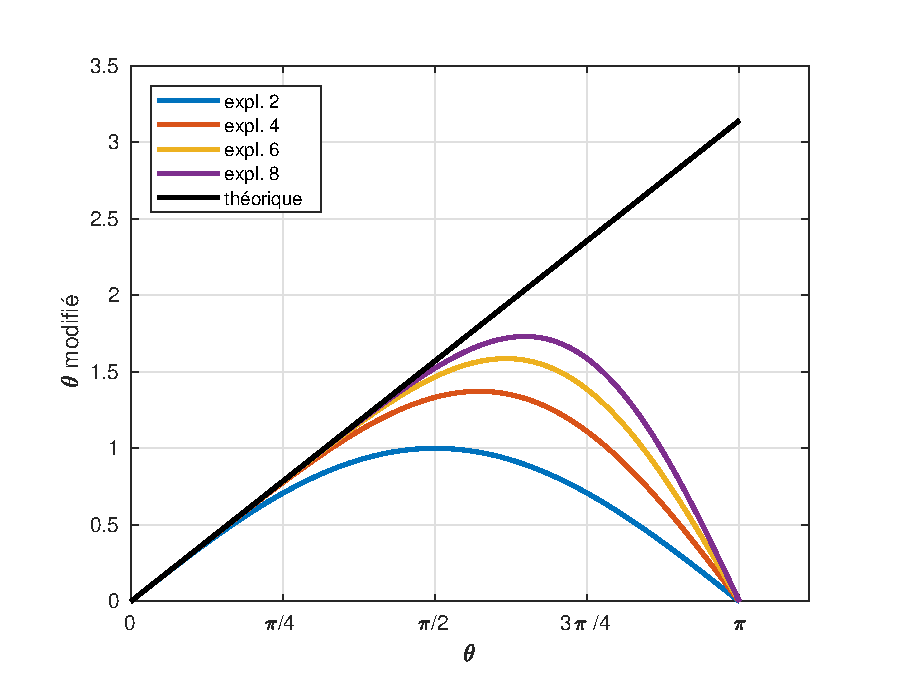
\includegraphics[scale=.6]{freq_classic.eps}
\end{center}
\caption{Représentation de $i Q_{2P}\left( \exp(i \theta) \right)$ en fonction de $\theta$ pour les schémas d'approximation explicites $\delta_{x,P}$ d'ordres 2, 4, 6 et 8.}
\label{fig:freq_classic}
\end{figure}

On définit $D_{2P} \in \mathbb{M}_N(\mathbb{R})$ la matrice associée à l'opérateur $\delta_{2P,x}$ :
\begin{equation}
D_{2P} = \dfrac{1}{h} Q_{2P}(T).
\end{equation}
La relation suivante est alors vérifiée
\begin{equation}
\vec_1(\delta_{2P,x} \mathfrak{u}) = D_{2P} \vec_1 ( \mathfrak{u} )
\end{equation}
pour tout $\mathfrak{u} \in l^2_{h,per}$.

Par exemple, le schéma centré d'ordre 2 $\delta_x = \delta_{2,x}$ est associée à la matrice
\begin{equation}
D_2 = \dfrac{1}{2h}
\begin{bmatrix}
0 & 1 &   &   &   & -1 \\ 
-1 & 0 & 1 &   & (0) &   \\ 
  & -1 & 0 & 1 &   &   \\ 
  &   & \ddots & \ddots & \ddots &   \\ 
  & (0) &   & -1 & 0 & 1 \\ 
1 &   &   &   & -1 & 0
\end{bmatrix} 
\end{equation}

\begin{proposition}
Les valeurs propres de $D_{2P}$ sont données par $\dfrac{1}{h}Q_{2P}(\omega^k)$ avec $-N/2 +1 \leq k \leq N/2$. Chaque valeur propre est associée à un vecteur propre $\vec_1{\mathfrak{u}^k}$.
\end{proposition}

\begin{proposition}
La matrice $D_{2P}$ est antisymétrique.
\end{proposition}

\begin{proof}
Montrons que $D_{2P}^T = - D_{2P}$ :
\begin{align*}
D_{2P}^T & = \dfrac{1}{h} Q_{2P}(T)^T \\
	& = \dfrac{1}{h} \left( \gsum_{j=1}^P \dfrac{a_j}{2j} (T^j - T^{N-j}) \right)^T\\
	& = \dfrac{1}{h}\gsum_{j=1}^P \dfrac{a_j}{2j} ((T^j)^T - (T^{N-j})^T) \\
	& = \dfrac{1}{h}\gsum_{j=1}^P \dfrac{a_j}{2j} (T^{N-j} - T^{j}) \\
	& = - \dfrac{1}{h} \gsum_{j=1}^P \dfrac{a_j}{2j} (T^j - T^{N-j}) \\
	& = - D_{2P}
\end{align*}
d'où le résultat.
\end{proof}





























\subsection{Opérateurs Hermitiens périodiques 1D}

Dans son article \cite{Lele1991}, S. K. Lele présente une méthode permettant d'approcher la dérivée en un point en ajoutant une partie implicite au schéma de la forme \eqref{eq:explicite_dx}. Dans ce chapitre, nous ne considérons que les schémas à 3 points implicites. Définissons l'opérateur $\sigma_{x}$ par :

\begin{equation}
(\sigma_{x} \mathfrak{u})_j = (1-2\beta) \mathfrak{u}_j + \beta \left( \mathfrak{u}_{j+1} + \mathfrak{u}_{j-1} \right)
\end{equation}

\begin{theoreme}
Si les coefficients réels $\beta$ et $(a_i)_{1 \leq i \leq P}$ sont solutions de 
\begin{equation}
\left\lbrace
\begin{array}{rcl}
\gsum_{p=1}^P a_p & = & 1 \\
\gsum_{p=1}^P a_p \dfrac{p^{2n}}{2n+1} & = & 2 \beta  \text{ pour } n=1,2,...P
\end{array}
\right.
\label{eq:hermitian_system}
\end{equation}
et si $u$ est une fonction de $\mathcal{C}^{2P+3}$, alors pour tout $0 \leq i \leq N-1$, on a 
\begin{equation}
(\delta_{2P,x} u^*)_i - (\sigma_{3,x} u'^*)_i = \\
h^{2P+2} \left( \gsum_{p=1}^P a_p  \dfrac{j^{2P+2} P}{(2P+3)!}  - \dfrac{2\beta}{(2P+2)!}   \right)u^{(2P+3)}(\rho)
\label{eq:eq_cons}
\end{equation}
avec $\rho \in [x_{i-P}, x_{i+P}]$.
\end{theoreme}

\begin{proof}
Soit $u : x \in \Omega \mapsto u(x) \in \mathbb{R}$ une fonction de classe $\mathcal{C}^{2P+3}( \Omega)$ et $u^*$ la fonction de grille correspondante.

On considère les développements de Taylor :
\begin{equation}
\begin{array}{rcl}
u(x_i + ph) & = & u(x_i) + p h u'(x_j) + \cdots + \dfrac{(ph)^k}{k!}u^{(k)}(x_i) + \cdots +\dfrac{(ph)^{2P+3}}{(2P+3)!} u^{(2P+3)}(\xi_p)\\
u(x_i - ph) & = & u(x_i) - p h u'(x_j) + \cdots + \dfrac{(-ph)^k}{k!}u^{(k)}(x_i) + \cdots +\dfrac{(-ph)^{2P+3}}{(2P+3)!} u^{(2P+3)}(\eta_p)
\end{array}
\end{equation}
avec $\xi_p \in [x_i, x_i+ph]$ et $\eta_p \in [x_i-ph, x_i]$. En combinant ces deux égalités, on a
\begin{equation}
\dfrac{\tau_pu^*_i - \tau_{-p} u^*_i}{2ph} = u'(x_i) + \cdots + \dfrac{(ph)^{k-1}(1 - (-1)^k)}{2 \cdot k!} u^{(k)}(x_i) + \cdots +\dfrac{(ph)^{2P+2}}{2(2P+3)!} \left( u^{(2P+3)}(\xi_p) + u^{(2P+3)}(\eta_p) \right)
\label{eq:preuve_herm1}
\end{equation}

D'autres part, on a 
\begin{equation}
(1-2\beta) u'^*_i + \beta \left( \tau_1 u'^*_{i} + \tau_{-1} u'^*_{i} \right) = u'^*_i +  \gsum_{k=1}^{2P+1} \beta \dfrac{h^{k}}{k!} \left( 1 + (-1)^k \right) u^{(k+1)}(x_i)+ \beta \dfrac{h^{2P+2}}{(2P+2)!} \left(u^{(2P+3)}(\varrho) + u^{(2P+3)}(\sigma) \right) 
\label{eq:preuve_herm2}
\end{equation}
avec $\varrho \in [x_i, x_i + h]$ et $\sigma \in [x_i, x_i - h]$. 

On remarque directement que \eqref{eq:preuve_herm2} et $\gsum_{p=0}^P a_p  \eqref{eq:preuve_herm1}$ coïncident pour les puissances de $h$ impaires. 

Pour les autres valeurs, l'égalité est vrai si les coefficients $a_p$ et $\beta$ sont solutions de \eqref{eq:hermitian_system}. L'erreur de troncature prend directement la forme 

\begin{multline}
(\delta_{2P,x} u^*)_i - (\sigma_{3,x} u'^*)_i = \\
h^{2P+2} \left( \gsum_{p=1}^P a_p  \dfrac{p^{2P+2}}{2(2P+3)!} \left( u^{(2P+3)}(\xi_j) + u^{(2P+3)}(\eta_j) \right) - \dfrac{\beta}{(2P+2)!} \left(u^{(2P+3)}(\varrho) + u^{(2P+3)}(\sigma) \right) \right)
\end{multline}
On conclut en utilisant le théorème des valeurs intermédiaires.
\end{proof}

\begin{proposition}
Le système \eqref{eq:hermitian_system} admet une unique solution.
\end{proposition}

\begin{proof}
TBA.
\end{proof}

\begin{proposition}
Les valeurs propres de $\sigma_x$ sont
\begin{equation}
R(\omega^k) \text{ avec } R(X) = (1-2 \beta) + \beta(X+X^{N-1}) \in \mathbb{R}_{N-1}[X] \text{ et } -N/2+1 \leq k \leq N/2.
\end{equation}
Le vecteur propre associé à $R(\omega^k)$ est $\mathfrak{u}^k$.
\end{proposition}

\begin{proof}
Conséquence de la proposition \ref{prop:eigen_Ptau}.
\end{proof}

\begin{corollaire}
L'opérateur $\sigma_x$ est inversible si
\begin{equation}
| \beta | < \dfrac{1}{4}.
\end{equation}
\end{corollaire}

\begin{definition}
On suppose que $\beta$ et $(a_p)_{1 \leq p \leq P}$ sont solutions de \eqref{eq:hermitian_system} et que $\beta < 1/4$, on définit l'\textit{opérateur hermitien} d'approximation de la dérivée première $\delta_x^H$ par 
\begin{equation}
\delta_{2P,x}^H = \sigma_x^{-1} \circ \delta_{2P,x}.
\end{equation}
\end{definition}

\begin{theoreme}
Si $u : x \in \Omega \mapsto u(x) \in \mathbb{R}$ est une fonction de classe $\mathcal{C}^{(2P+3)}$.
Alors 
\begin{equation}
\| u'^* - \delta_{2P,x}^H u^* \|_{\infty} \leq C h^{2P+2} \| u^{(2P+3)} \|_{\infty}
\end{equation}
où $C$ est une constante indépendante de $u$.
\label{th:consistence_herm2}
\end{theoreme}

\begin{proof}
Par calcul immédiat, on a :
\begin{equation}
\begin{array}{rcl}
\|  u'^* - \delta_{2P,x}^H u^* \|_{\infty} &=& \| \sigma_{3,x}^{-1} \circ \left( \sigma_{3,x} u'^*  - \delta_{2P,x}u^*\right) \|_{\infty}\\
                                      &\leq& \| \sigma_{3,x}^{-1} \|_{\infty} \| \sigma_{3,x} u'^*  - \delta_{2P,x}u^*\|_{\infty}\\
                                      &\leq& C h^{2P+2}  \| u^{(2P+3)} \|_{\infty}
\end{array}
\end{equation}
en utilisant $\sigma_{3,x}$ inversible et l'équation \eqref{eq:eq_cons}.
\end{proof}


Quelques exemples de schémas hermitiens sont donnés dans le corollaire suivant.

\begin{corollaire}
Soit $u : x \in \Omega \mapsto u(x) \in \mathbb{R}$ alors 
\begin{itemize}
\item Si $u \in \mathcal{C}^{5}(\Omega)$ alors 
\begin{equation}
\begin{array}{rcl}
\sigma_{x} &=& \dfrac{4}{6} id + \dfrac{1}{6} \left( \tau_1 + \tau_{-1} \right)\\
\delta_{2,x} &=& \dfrac{\tau_1 - \tau_{-1}}{2h} \\ 
\end{array}
\label{eq:comp4}
\end{equation}
et $\delta^H_{2,x} = \sigma_x^{-1} \circ \delta_{2,x}$ définit un opérateur d'approximation de la dérivée première à l'ordre 4,

\item Si $u \in \mathcal{C}^{7}(\Omega)$ alors 
\begin{equation}
\begin{array}{rcl}
\sigma_{x} &=& \dfrac{1}{2} id + \dfrac{1}{4}\left( \tau_1 + \tau_{-1} \right) \\
\delta_{4,x} &=& \dfrac{5}{6} \dfrac{\tau_1 - \tau_{-1}}{2h} + \dfrac{1}{6} \dfrac{\tau_2 - \tau_{-2}}{4h}\\ 
\end{array}
\label{eq:comp6}
\end{equation}
et $\delta^H_{4,x} = \sigma_{x}^{-1} \circ \delta_{4,x}$ définit un opérateur d'approximation de la dérivée première à l'ordre 6,


\item Si $u \in \mathcal{C}^{9}(\Omega)$ alors 
\begin{equation}
\begin{array}{rcl}
\sigma_{x} &=& \dfrac{4}{7} id + \dfrac{3}{14}\left( \tau_1 + \tau_{-1} \right) \\
\delta_{6,x} &=& \dfrac{25}{28} \dfrac{\tau_1 - \tau_{-1}}{2h} + \dfrac{4}{35} \dfrac{\tau_2 - \tau_{-2}}{4h} - \dfrac{1}{140} \dfrac{\tau_3 - \tau_{-3}}{6h} \\ 
\end{array}
\label{eq:comp8}
\end{equation}
et $\delta^H_{6,x} = \sigma_{x}^{-1} \circ \delta_{6,x}$ définit un opérateur d'approximation de la dérivée première à l'ordre 8.

\end{itemize}
\end{corollaire}

Comme les opérateurs $\sigma_x$ et $\sigma_{2P,x}$ s’expriment en fonction de $\tau$, ils commutent tout comme $\sigma_x^{-1}$ et $\sigma_{2P,x}$:
\begin{equation}
\delta_{2P,x}^H = \sigma_x^{-1} \circ \delta_{2P,x} = \delta_{2P,x} \circ \sigma_x^{-1}
\end{equation}
Il existe donc une fraction rationnelle $Q_{2P}^H \in \mathbb{R}(X)$ telle que 
\begin{equation}
\delta_{2P,x}^H = \dfrac{1}{h} Q_{2P}^H( \tau ).
\end{equation}
Cette fraction rationnelle est donnée par
\begin{equation}
Q_{2P}^H(X) = \dfrac{Q_{2P}(X)}{R(X)} = \dfrac{\gsum_{j=1}^P \dfrac{a_j}{2j} (X^j - X^{N-j})}{(1-2\beta) + \beta ( X + X^{N-1})}.
\end{equation}

Les valeurs propres de $\delta_{2P,x}^H$ s'expriment grâce à $Q_{2P}^H(X)$.

\begin{proposition}
Les valeurs propres de $\delta_{2P,x}^H$ sont 
\begin{equation}
\dfrac{1}{h} Q_{2P}^H (\omega^k)
\end{equation}
où $-N/2+1 \leq k \leq N/2$. $\omega^k$ est associé à la fonction propre $\mathfrak{u}^k$.
\label{prop:eigen_mat_hermitien}
\end{proposition}

Comme pour les schémas aux différences finies classiques, si on pose \begin{equation}
\theta = \dfrac{2 \pi k}{N},
\end{equation}
on montre directement que
\begin{equation}
\theta - i Q_{2P}^H ( e^{i \theta} ) = \mathcal{O} \left( h^{2P+3} \right).
\end{equation}

De plus, on note que $i Q_{2P}^H(e^{i0}) = 0$ et $i Q_{2P}^H(e^{i\pi}) = 0 \neq \pi$. Comme pour les schémas de la forme $\delta_{2P,x}$, on compare $\theta \in [0 , \pi] \mapsto - i Q_{2P}^H(e^{i \theta})$ et $\theta$ en Fig. \ref{fig:freq_herm}.
\begin{figure}[htbp]
\begin{center}
\includegraphics[scale=.6]{compact_freq.png}
\end{center}
\caption{Représentation de $i Q_{2P}^H \left( e^{i \theta} \right)$ en fonction de $\theta$ pour les schémas d'approximation hermitien $\delta_{2P,x}^H$ d'ordres 2, 4, 6 et 8. Les courbes en pointillés représentent les fonctions $i Q_{2P}\left( e^{i \theta} \right)$ associées aux opérateurs d'approximations $\delta_{2P,x}$.}
\label{fig:freq_herm}
\end{figure}
On constate que les schémas hermitiens représentent mieux les fréquences que les schémas classiques au même ordre de précision. Comme pour les schémas $\delta_{2P,x}$, augmenter l'ordre permet d'assurer une meilleure représentation des hautes fréquences.

D'une manière générale, les schémas hermitiens permettent d'assurer une bonne précision aussi bien en terme d'ordre qu'en terme de représentation des fréquences. Les schémas hermitiens permettent d'assurer de bons résultats mais nécessitent le calcul de l'inverse de l'opérateur $\sigma_x$. Le coût en calcul est donc, a priori, plus important.

Dans la pratique, le calcul se fait au niveau matriciel. En effet, on construit la matrice $P$ par
\begin{align}
P & = R(T) \\
  & = \begin{bmatrix}
  1 - 2 \beta & \beta &   &   & \beta \\ 
  \beta & 1 - 2 \beta & \beta & (0) &   \\ 
    & \ddots & \ddots & \ddots &   \\ 
    & (0) & \beta & 1 - 2 \beta & \beta \\ 
  \beta &   &   & \beta & 1 - 2 \beta
  \end{bmatrix} 
\end{align}
et l'on a 
\begin{equation}
\vec_1 (\sigma_x \mathfrak{u}) = P \vec_1 (\mathfrak{u}).
\end{equation}

Les valeurs propres de $P$ sont connues et données par la proposition \ref{prop:eigen_P(T)}.
\begin{proposition}
Les valeurs propres de $P$ sont 
\begin{equation}
R(\omega^k)
\end{equation}
avec $-N/2+1 \leq k \leq N/2$. Chaque valeur propre est associé au vecteur propre $\vec_1( \mathfrak{u}^k )$.
\end{proposition}

$P$ est inversible si $|\beta |<1/4$ et trivialement symétrique. 
De la même manière, on a déjà vu que 
\begin{equation}
D_{2P} = \dfrac{1}{h} Q_{2P}(T)
\end{equation}
donc 
\begin{equation}
\vec_1 (\delta_{2P,x} \mathfrak{u}) = D_{2P} \vec_1 (\mathfrak{u}).
\end{equation}

Le calcul de $\delta^H_{2P,x} \mathfrak{u}$ se fait par la résolution du système
\begin{equation}
P \vec_1 (\delta_{2P,x}^H \mathfrak{u}) = D_{2P} \vec_1 (\mathfrak{u})
\end{equation}

La solution de ce système peut être calculée grâce à la formule de Shermann-Morisson-Woodbury couplé à un solveur tridiagonal comme l'algorithme de Thomas.

\begin{proposition}
\textbf{(Formule de Shermann-Morisson-Woodbury)} Soient $A, B \in \mathbb{M}_N \left(\mathbb{R} \right)$ deux matrices inversibles telles que 
\begin{equation}
A = B + R S^T,
\end{equation}
avec $R$ et $S$ deux matrices de $\mathbb{M}_{N,n} \left(\mathbb{R} \right)$ avec $n \leq N$.
Alors l'inverse de $A$ peut s'écrire
\begin{equation}
A^{-1} = B^{-1} - B^{-1} R \left( Id + S^T B^{-1} R  \right)^{-1} S^T B^{-1}.
\label{eq:SMW}
\end{equation}
\end{proposition}

\begin{proof}
Il suffit de vérifier que 
\begin{equation}
\left( B + R S^T \right) \left( B^{-1} - B^{-1} R \left( Id + S^T B^{-1} R  \right)^{-1} S^T B^{-1} \right) = Id.
\end{equation}
\end{proof}

Dans le cas où $n \lll N$, $A$ est une petite perturbation de la matrice $B$ de la forme 
\begin{equation}
A = B + \delta B
\end{equation}
avec $\rang  (\delta B) $ "petit". Si on peut facilement calculer l'inverse de $B$ la formule de Shermann-Morisson-Woodbury \eqref{eq:SMW} donne un algorithme efficace de résolution du système
\begin{equation}
A X = b.
\end{equation} 

\begin{center}
\begin{minipage}[H]{12cm}
  \begin{algorithm}[H]
    \caption{: Algorithme de Shermann-Morisson-Woodbury}\label{alg:SMW}
    \begin{algorithmic}[1]
	\State Calcul de $V_1 = B^{-1} b$,
	\State Calcul de $V_2 = S^T V_1$,
	\State Calcul de $V_3 = (Id + S^T B^{-1}R)^{-1} V_2$ (résolution d'un système de petite taille),
	\State Calcul de $V_4 = R V_3$,
	\State Calcul de $V_5 = B^{-1} V_4$,
	\State Calcul de $X = V_1 - V_5$.
    \end{algorithmic}
    \end{algorithm}
\end{minipage}
\end{center}

\begin{proposition}
Soit $P$ et $\tilde{P}$ les matrice donnée par 
\begin{equation}
P = \begin{bmatrix}
  1 - 2 \beta & \beta &   &   & \beta \\ 
  \beta & 1 - 2 \beta & \beta & (0) &   \\ 
    & \ddots & \ddots & \ddots &   \\ 
    & (0) & \beta & 1 - 2 \beta & \beta \\ 
  \beta &   &   & \beta & 1 - 2 \beta
  \end{bmatrix}  \text{ et }
\tilde{P} = 
\begin{bmatrix}
  1 - 2 \beta & \beta &   &   &  \\ 
  \beta & 1 - 2 \beta & \beta & (0) &   \\ 
    & \ddots & \ddots & \ddots &   \\ 
    & (0) & \beta & 1 - 2 \beta & \beta \\ 
   &   &   & \beta & 1 - 2 \beta
  \end{bmatrix} .
\end{equation}
Alors 
\begin{equation}
P = \tilde{P} + R S^T
\end{equation} 
avec 
\begin{equation}
R = \dfrac{1}{6}\begin{bmatrix}
1 & 0 \\ 
0 & \vdots \\ 
\vdots & \vdots \\ 
\vdots & 0 \\ 
0 & 1
\end{bmatrix} \text{ et } 
S = \begin{bmatrix}
0 & 1 \\ 
\vdots & 0 \\ 
\vdots & \vdots \\ 
0 & \vdots \\ 
1 & 0
\end{bmatrix} 
\end{equation}
\end{proposition}

il découle l'algorithme le calcul de $\vec_1 (\delta_{2P,x}^H \mathfrak{u}) = P^{-1}D_{2P} \vec_1 (\mathfrak{u})$ donné par

\begin{center}
\begin{minipage}[H]{12cm}
  \begin{algorithm}[H]
    \caption{: Calcul Hermitien}\label{alg:SH}
    \begin{algorithmic}[1]
    \State Calcul de $b = D_{2P} \vec_1 (\mathfrak{u})$,
	\State Calcul de $V_1 = \tilde{P}^{-1} b$,
	\State Calcul de $V_2 = S^T V_1$,
	\State Calcul de $V_3 = (Id + S^T \tilde{P}^{-1}R)^{-1} V_2$ (résolution d'un système de taille $2 \times 2$),
	\State Calcul de $V_4 = R V_3$,
	\State Calcul de $V_5 = \tilde{P}^{-1} V_4$,
	\State Calcul de $\vec_1 (\delta_{2P,x}^H \mathfrak{u}) = V_1 - V_5$.
    \end{algorithmic}
    \end{algorithm}
\end{minipage}
\end{center}
La matrice $\tilde{P}$ étant tridiagonale, elle peut être inversée simplement en utilisant l'algorithme de Thomas. Le calcul de $U'$ a un coût du même ordre de grandeur que le coût de résolution de $\tilde{P}X = b$. Concernant la matrice de calcul du schéma hermitien, un certain nombre de résultats sont vérifiés.

\begin{proposition}
Les matrices $D_{2P}$, $P$ et $P^{-1}$ commutent.
\end{proposition}

\begin{proof}
Consèquence de l'écriture de ces matrices à l'aide de $T$.
\end{proof}

\begin{proposition}
La matrice $P^{-1}D_{2P}$ est antisymétrique.
\end{proposition}

\begin{proof}
Par calcul immédiat, on a :
\begin{equation}
(P^{-1}D_{2P})^T = D_{2P}^T P^{-T} = - D_{2P} P^{-1} = - P^{-1} D_{2P}.
\end{equation}
car $D_{2P}$ est antisymétrique et $P$ est symétrique (donc $P^{-1}$ aussi). 
\end{proof}

























\subsection{Opérateur de filtrage}


Lors de la discrétisation via un schéma aux différences finies et suite à la discrétisation en temps, des oscillations parasites du type "+1/-1" peuvent apparaître. Il s'agit de phénomènes haute fréquences qui peuvent provoquer des instabilités numériques. 

Si $\mathfrak{u}$ est une fonction de grille périodique, on note le filtre passe-bas $\mathcal{F}\mathfrak{u}$. Dans la pratique, nous cherchons $\mathcal{F}$ sous la forme 

\begin{equation}
\mathcal{F} = \gsum_{k=0}^F a_k \dfrac{\tau^k + \tau^{-k}}{2} = S(\tau)
\label{eq:ftr}
\end{equation}

avec $S \in \mathbb{R}_{N-1}[X]$ et 
\begin{equation}
S(X) = \gsum_{k=0}^F a_k \dfrac{X^k + X^{N-k}}{2}
\end{equation}
Les coefficients $(a_k)_{0 \leq k \leq F}$ sont déterminés de manière à supprimer les phénomènes oscillants hautes fréquences (figure \ref{fig:hf_waves}) de la formes $\mathfrak{u}$ avec 
\begin{equation}
\mathfrak{u}_j = (-1)^j
\end{equation}

\begin{figure}[htbp]
\begin{center}
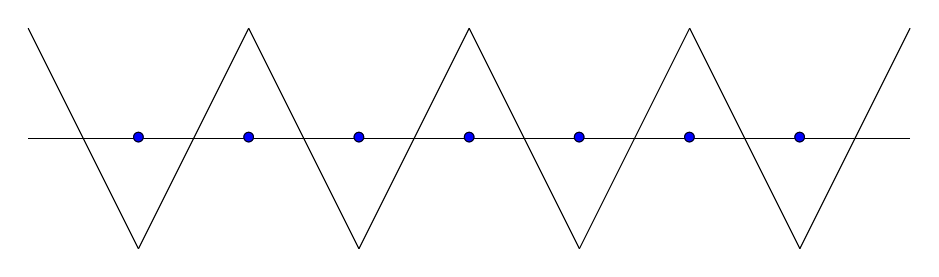
\begin{tikzpicture}[scale=1.4]
	\draw (-4,1) -- (-3,-1) ;
	\draw (-3,-1) -- (-2,1) ;
	\draw (-2,1) -- (-1,-1) ;
	\draw (-1,-1) -- (0,1) ;
	\draw (0,1) -- (1,-1) ;
	\draw (1,-1) -- (2,1) ;
	\draw (2,1) -- (3,-1) ;
	\draw (3,-1) -- (4,1) ;
	
	\draw (4,0) -- (-4,0) ;
	\foreach \k in {-3,...,3}
		{\draw  (\k,0) node[color=blue] {$\bullet$} ;
	   	\draw (\k,0) node {$\circ$} ;
	   	}
\end{tikzpicture}
\end{center}
\caption{Ondes de type "+1/-1".}
\label{fig:hf_waves}
\end{figure}


En considérant cette fonction de grille, on cherche $(a_k)_{0\leq k \leq F}$ tels que $\mathcal{F} \mathfrak{u} = \mathfrak{0}$, soit :
\begin{equation}
\mathcal{F}\mathfrak{u}_i = \gsum_{k=0}^F a_k \dfrac{\mathfrak{u}_{i+k} + \mathfrak{u}_{i-k}}{2} = \gsum_{k=0}^F a_k  \dfrac{(-1)^{i+k} + (-1)^{i-k}}{2} = 0.
\end{equation}
Cette équation est équivalente à 
\begin{equation}
\gsum_{k=0}^F a_k (-1)^k = 0
\label{eq:ftr_ftrcond}
\end{equation}
La relation \eqref{eq:ftr_ftrcond} nous donne une condition alors qu'il y a $F+1$ paramètres à déterminer. Il reste $F$ degrés de libertés dans l'opérateur de filtrage. Le choix qui est fait est de maximiser l'ordre du filtrage de manière à perturber un minimum la donnée initiale tout en supprimant les ondes parasites.

Le filtre doit conserver les très basses fréquences, lorsque $\mathfrak{u} = \mathfrak{1}$, on doit alors $\mathcal{F}\mathfrak{u} = \mathfrak{1}$.
C'est à dire que les coefficients $(a_k)_{0 \leq k \leq F}$ vérifient la relation de consistance
\begin{equation}
\gsum_{k=0}^F a_k = 1
\label{eq:ftr_conscond}
\end{equation}

Enfin, on remarque que si $u : x \in \Omega \mapsto u(x) \in \mathbb{R}$ et si $u^*$ est la fonction de grille associée à $u$, alors on a 
\begin{equation}
\begin{array}{rcl}
u(x_i + kh) & = & u(x_i) + p k u'(x_j) + \cdots + \dfrac{(kh)^l}{l!}u^{(l)}(x_i) + \cdots +\dfrac{(kh)^{2F}}{2F!} u^{(2F)}(\xi_k)\\
u(x_i - kh) & = & u(x_i) - p k u'(x_j) + \cdots + \dfrac{(-kh)^l}{l!}u^{(l)}(x_i) + \cdots +\dfrac{(-kh)^{2F}}{2F!} u^{(2F)}(\eta_k)
\end{array}
\end{equation}
avec $\xi_k \in [x_i, x_i+kh]$ et $\eta_k \in [x_i-kh, x_i]$. Alors par combinaison linéaire en considérant \eqref{eq:ftr_conscond} vérifiée, 
\begin{equation}
\mathcal{F}u^* - u^* = \gsum_{l=1}^{2F-1} \gsum_{k=0}^F \dfrac{a_k}{2} \underbrace{\dfrac{(kh)^l + (-kh)^l}{l!}}_{=0 \text{ pour } l \text{ impair.}}u^{(l)}(x_i) + \gsum_{k=0}^F \dfrac{a_k}{2}\dfrac{(kh)^{2F}}{2F!} \left( u^{(2F)}(\xi_k) + u^{(2F)}(\eta_k) \right)
\end{equation}
Ainsi, la condition de précision est 
\begin{equation}
\gsum_{k=0}^F a_k k^{2l} = 0 \text{ pour } 1 \leq l \leq F-1.
\label{eq:ftr_prescond}
\end{equation}

\begin{theoreme}
Soit $F \in \mathbb{N}^{\star}$. Il existe un unique $(a_k)_{0 \leq k \leq F}$ tel que $\mathcal{F}$ soit à la fois consistant en vérifiant \eqref{eq:ftr_conscond}, précis en vérifiant \eqref{eq:ftr_prescond} et soit un filtre passe bas en satisfesant \eqref{eq:ftr_ftrcond}. L'erreur de troncature du filtre est alors donnée par 
\begin{equation}
\mathcal{F}u^* - u^* = h^{2F} \gsum_{k=0}^F \dfrac{a_k}{2} \dfrac{k^{2F}}{2F!} \left( u^{(2F)}(\xi_k) + u^{(2F)}(\eta_k) \right).
\end{equation}
\label{prop:filter_def}
\end{theoreme}

\begin{proof}
La forme de l'erreur de troncature a déjà été vue, il reste à prouver l'unicité.

Après avoir retiré \eqref{eq:ftr_ftrcond} à \eqref{eq:ftr_conscond}, dire qu'il existe une unique $(a_j)_{0 \leq j \leq J}$ satisfesant les conditions est équivalent à dire que la matrice

\begin{equation}
A=\begin{bmatrix}
1 &  1  &  1  &  1  &  1  &  1  & \cdots\\  
0 &  2  &  0  &  2  &  0  & 2  & \cdots\\
0 &  1  & 2^2 & 3^2 & 4^2 & 5^2 & \cdots\\
0 &  1  & 2^4 & 3^4 & 4^4 & 5^4 & \cdots\\
0 &  1  & 2^6 & 3^6 & 4^6 & 5^6 & \cdots\\
&&& \vdots &  \vdots &
\end{bmatrix} \in \mathbb{M}_{J+1} \left( \mathbb{R} \right)
\end{equation}
est inversible car $a = [a_0, a_1, \cdots, a_J]^T$ est solution de 
\begin{equation}
A a = e_1
\end{equation}
avec $e = [1,1/2, 0,\cdots,0]^T$. En développant la seconde ligne de $A$, on a
\begin{equation}
\det ( A ) = \begin{vmatrix} 
2  &  0  &  2  &  0  & 2  & \cdots\\
1  & 2^2 & 3^2 & 4^2 & 5^2 & \cdots\\
1  & 2^4 & 3^4 & 4^4 & 5^4 & \cdots\\
1  & 2^6 & 3^6 & 4^6 & 5^6 & \cdots\\
& & \vdots &  \vdots &
\end{vmatrix} = 2 \sum_{k=1}^{\lfloor\frac{F-1}{2}\rfloor} \Delta_{2k+1}
\end{equation}
avec $\Delta_k$ donné par
\begin{equation}
\Delta_k = \begin{vmatrix} 
1 & 2^2 & \cdots & (k-1)^2 & (k+1)^2 & \cdots\\
1 & 2^4 & \cdots & (k-1)^4 & (k+1)^4 & \cdots\\
1 & 2^6 & \cdots & (k-1)^6 & (k+1)^6 & \cdots\\
&&& \vdots &  \vdots &
\end{vmatrix} = \dfrac{((F-1)!)^2}{k^2} \begin{vmatrix} 
1 & 1 & \cdots & 1 & 1 & \cdots\\
1 & (2^2)^1 & \cdots & ((k-1)^2)^1 & ((k+1)^2)^1 & \cdots\\
1 & (2^2)^2 & \cdots & ((k-1)^2)^2 & ((k+1)^2)^2 & \cdots\\
&&& \vdots &  \vdots &
\end{vmatrix}
\end{equation}
On reconnaît un déterminant de Van-Der-Monde, donc $\Delta_k = \prod_{1 \leq i < j \leq F-1} \left( \alpha_j - \alpha_i \right)$, avec 
\begin{equation}
\alpha_j = \left\lbrace
\begin{array}{ll}
j^2 & \text{ avec } 1 \leq j \leq k-1\\
(j+1)^2 & \text{ avec } k \leq j \leq J-2\\
\end{array}
\right.
\end{equation}
Si $i<j$, on a $\alpha_i < \alpha_j$, donc $\Delta_k>0$ et $\det A$ est une somme de déterminants tous strictements positifs donc $\det A > 0$. $A$ est inversible et le résultat est prouvé.
\end{proof}
Quelques filtres particuliers sont donnés dans la table \ref{tab:filter} en fonction de leur ordre de précision.
\begin{table}[htbp]
\begin{center}
\begin{tabular}{|c||cccccc|}
\hline
\textbf{Ordre de précision} & $a_0$ & $a_1$ & $a_2$ & $a_3$ & $a_4$ & $a_5$ \\
\hline \hline
$2$ & $1/2$ & $1/2$ & & & & \\
\hline
$4$ & $10/16$ & $8/16$ & $-2/16$ & & & \\
\hline
$6$ & $44/64$ & $30/64$ & $-12/64$ & $2/64$ & & \\
\hline
$8$ & $186/256$ & $112/256$ & $-56/256$ & $16/256$ & $-2/256$ & \\
\hline
$10$ & $772/1024$ & $420/1024$ & $-240/1024$ & $90/1024$ & $-20/1024$ & $2/1024$ \\
\hline
\end{tabular}
\end{center}
\caption{Exemples de filtres de la forme \eqref{eq:ftr} et leurs ordres de précision.}
\label{tab:filter}
\end{table}
Dans la suite, nous supposerons que $(a_k)_{0 \leq k \leq F}$ satisfait les conditions \eqref{eq:ftr_conscond}, \eqref{eq:ftr_prescond} et \eqref{eq:ftr_ftrcond}.
Les valeurs propres et fonctions propres de $\mathcal{F}$ sont issues de la proposition \ref{prop:eigen_Ptau}.

\begin{theoreme}
Les valeurs propres de $\mathcal{F}$ sont données par $\beta^k$ avec 
\begin{equation}
\beta^k = S(\omega^k) = \gsum_{f=0}^F a_k \cos \left( \dfrac{2 \pi k f}{N} \right)
\end{equation}
pour tout $0 \leq k \leq N-1$, $\beta^k$ est associé à la fonction propre $\mathfrak{u}^k$.
\end{theoreme}

On définit le \textit{symbole} du filtre $\mathcal{F}$ par la fonction $\beta : \theta \in [0, \pi] \mapsto \beta(\theta) \in \mathbb{R}$ donnée par :
\begin{equation}
\beta( \theta ) = \gsum_{f=0}^F a_k \cos \left( f \theta \right) = S(e^{i \theta}).
\end{equation}

\begin{proposition}
Il existe un unique polynôme $P$ de degré $F$ tel que 
\begin{equation}
\beta(\theta) = P(\cos \theta )
\end{equation}
De plus,
\begin{equation}
P(x) = 1 -\dfrac{1}{(-2)^F} (X - 1)^F.
\end{equation}
\end{proposition}

\begin{proof}
Soit $\theta \in [0, \pi]$, 
\begin{equation}
\beta(\theta) = \gsum_{f=0}^F a_f \cos \left( f \theta \right) = \gsum_{f=0}^F a_f T_f ( \cos \theta )
\end{equation}
où $T_f \in \mathbb{R}_f [X]$ est le $k-$ieme polynome de Tchebytchev. 
Ainsi il existe $P \in \mathbb{R}_F [x]$ tel que $\beta( \theta ) = P( \cos \theta )$. Ce polynôme est unique. Montrons que 
\begin{equation}
P(x) = 1 -\dfrac{1}{(-2)^F} (X - 1)^F.
\end{equation}
convient.

\begin{itemize}
\item on montre facilement que 
\begin{equation}
P( \cos 0 ) = 1 -\dfrac{1}{(-2)^F} (\cos 0 - 1)^F = 1,
\end{equation}
de même,
\begin{equation}
P( \cos \pi ) = 1 -\dfrac{1}{(-2)^F} (\cos \pi - 1)^F 1 -\dfrac{(-2)^F}{(-2)^F} = 0.
\end{equation}
\item On rappelle la formule de Fàa Di Bruno permettant de calculer la dérivée $n-$ième d'une composée. Si $f$ et $g$ sont des fonctions régulières, on a 
\begin{equation}
\dfrac{d^n}{dx^n} \left( f \circ g \right)(x) = \gsum_{k=1}^n f^{(k)}\left( g(x) \right) B_{n,k}\left( g'(x), g''(x), \cdots , g^{n-k+1}(x) \right)
\end{equation}
où $B_{n,k}$ est un polynôme de Bell. En utilisant cette formule avec $f = P$ et $g = \cos$, évaluée en $\theta = 0$, on montre que :
\begin{equation}
\dfrac{d^n}{d\theta^n} \left( P \circ \cos \right)(0) = \gsum_{k=1}^n P^{(k)}\left(1\right) B_{n,k}\left( -1,0,1,0, \cdots\right)
\end{equation}
Or, $P^{(k)}\left(1\right) = 0$ pour tout $k \geq 1$. Donc 
\begin{equation}
\dfrac{d^n}{d\theta^n} \left( P \circ \cos \right)(0) = 0
\end{equation}
\end{itemize}
Le polynôme $P$ convient et 
\begin{equation}
\beta( \theta ) = 1 - \dfrac{1}{(-2)^F}(\cos \theta -1)^F.
\end{equation}
\end{proof}

\begin{proposition}
Pour tout $\theta \in [0, \pi]$, on a 
\begin{equation}
0 \leq \beta ( \theta ) \leq 1
\end{equation}
\end{proposition}

\begin{proof}
Supposons qu'il existe $\theta \in [0, \pi]$ tel que $\beta(\theta) < 0$ ou $\beta(\theta) > 1$. Comme $\beta(0)=1$ et $\beta(\pi) = 0$, il existe $\tilde{\theta} \in ]0, \pi[$ tel que 
\begin{equation}
\beta'(\tilde{\theta}) = - \sin \tilde{\theta} P'(\cos \tilde{\theta} ) = 0
\end{equation}
Or $\sin \tilde{\theta} \neq 0$ pour $\tilde{\theta} \in ]0, \pi[$.
De plus, 
\begin{equation}
P'(X) = \dfrac{F}{(-2)^F}(X-1)^{F-1}
\end{equation}
donc en prenant $X = \cos \tilde{\theta}$,
\begin{equation*}
P'(X) = 0 \Leftrightarrow \cos \tilde{\theta} = 1
\end{equation*}
Ce qui est impossible pour $\tilde{\theta} \in ]0, \pi[$. Donc par l'absurde, le résultat est vérifié.
\end{proof}

La fonction $\beta$ permet de considérer le comportement du filtre sur les différentes fréquences $\theta \in [0, \pi]$. Les basses fréquences sont bien conservées alors que les hautes fréquences ($\theta$ proche de $\pi$) sont atténuées. Cette observation est visible sur la figure \ref{fig:freq_filter} représentant la fonction $\beta : \theta \mapsto \beta(\theta)$ associée aux filtres d'ordre 2, 4, 6, 8 et 10. 

\begin{figure}[htbp]
\begin{center}
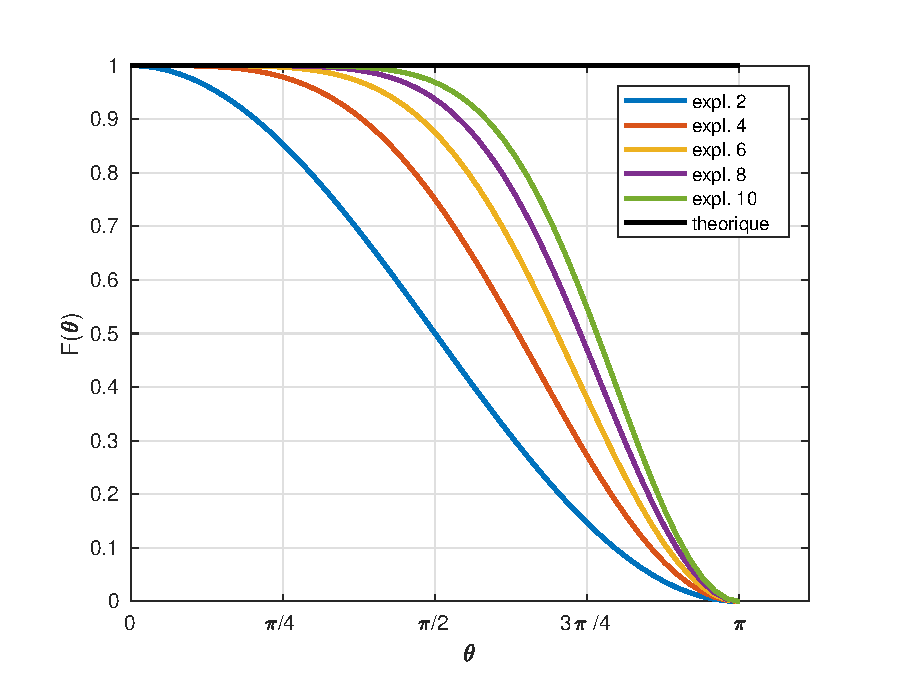
\includegraphics[scale=0.7]{freq_filter.eps}
\end{center}
\caption{Fonction d'amplification $\beta$ pour les filtres explicites d'ordre 2, 4, 6, 8 et 10.}
\label{fig:freq_filter}
\end{figure}
Comme on s'y attendais, un filtre d'ordre élevé laisse passer un plus grand nombre de basses fréquences. Dans le tableau \ref{tab:filter_095}, on représente la fréquence $\theta_{0.95}$ maximale qui est conservée à $95\%$. Comme la fonction $\beta$ est strictement décroissante et continue sur $[0,\pi]$, c'est une bijection de $[0,\pi]$ dans $[0,1]$ et on a 
\begin{equation}
\theta_{0.95} = \beta^{-1}(0.95)= \arccos \left[ 1-2 (0.05)^{1/F} \right].
\end{equation}

\begin{table}
\begin{center}
\begin{tabular}{|c||c|}
\hline
\textbf{Ordre du filtre} & \textbf{Fréquence conservée à } $95\%$\\
\hline
\hline
$10$&$1.6695$\\
$8$&$1.5165$\\
$6$&$1.3045$\\
$4$&$0.9851$\\
$2$&$0.4510$\\
\hline
\end{tabular}
\end{center}
\caption{Fréquence conservée à $95\%$ en fonction de l'ordre du filtre.}
\label{tab:filter_095}
\end{table}

La fonction $F \mapsto \theta_{0.95} = \beta^{-1}(0.95)$ est croissante, ce qui confirme que lorsque l'ordre de précision croit, $\theta_{0.95}$ croit et le filtre conserve un plus grand nombre de fréquences. De plus, 
\begin{equation}
\lim_{F \rightarrow +\infty} \theta_{0.95} = \pi.
\end{equation}
Ce qui confirme la prise en compte d'un grand nombre de fréquence lorsque l'on augmente l'ordre du filtre. Cependant lorsque l'ordre du filtre augmente, l'effet de filtrage des hautes fréquences diminue.

Le filtre utilisé est linéaire et agit sur les composantes des fonctions de grilles. Il existe $M \in \mathbb{M}_N \left( \mathbb{R} \right)$ la matrice associée au filtrage des données en dimension 1 telle que
\begin{equation}
\mathcal{F} \mathfrak{u} = M \mathfrak{u}
\end{equation}
et la matrice $M$ est donnée par
\begin{equation}
M = S(T).
\end{equation}

\begin{proposition}
La matrice $M$ est symétrique :
\begin{equation}
M = M^T.
\end{equation}
\end{proposition}
































\section{Opérateurs aux différences en dimension 2}


\subsection{Notations}
\label{sec:notation_2D}

En dimension 2, les notations sont analogues de celles utilisées en dimension 1. On se limite au cas d'une géométrie carrée. Si $a$ et $b$ sont des réels positifs, nous notons $\Omega = [a,b]^2$. Chaque côté du carré est de longueur $L=b-a$. 
Soient $u$ et $v$ deux fonctions de $\Omega$ dans $\mathbb{R}$. On note le produit scalaire dans $L^2 ( \Omega )$
\begin{equation}
(u,v) = \gint_{\Omega} u(x,y) v(x,y) dx dy.
\end{equation}
La norme associée est :
\begin{equation}
\| u \|_{L^2(\Omega)} = \sqrt{(u,v)}. 
\end{equation}
On note également
\begin{equation}
\| u \|_{L^{\infty} ( \Omega )} = \max_{(x,y) \in \Omega} |u(x,y)|.
\end{equation}
Pour alléger les notations nous notons ces deux normes $\| u \|_{L^2}$ et $\| u \|_{L^{\infty}}$.

Dans le domaine $\Omega$, la grille est constituée des points $(x_i,y_j)_{0 \leq i,j \leq N}$ où $N \geq 1$ avec $a = x_0 < x_1 < \ldots < x_N = b$ et $a = y_0 < y_1 < \ldots < y_N = b$. Le pas d'espace $h$ est fixe et donné par $h = \frac{L}{N}$. Les points de grilles sont $(x_i, y_j)$ avec 
\begin{equation}
\left\lbrace\begin{array}{rcl}
x_i & = & a + i h \\
y_j & = & a + j h 
\end{array}\right. \text{ avec } 0 \leq i,j \leq N.
\end{equation}

Les points $(x_i,y_j)_{0 \leq i,j \leq N}$ sont de deux types (voir figure \ref{fig:maillage2D}) :
\begin{itemize}
\item Les points de bords $(x_i, y_j)$ avec
\begin{equation}
i \in \left\lbrace 0 , N \right\rbrace \text{ ou } j \in \left\lbrace 0 , N \right\rbrace,
\end{equation}
\item les points intérieurs $(x_i, y_j)$ avec
\begin{equation}
1 \leq i,j \leq N-1.
\end{equation}
\end{itemize}



\begin{figure}[htbp]
\begin{center}
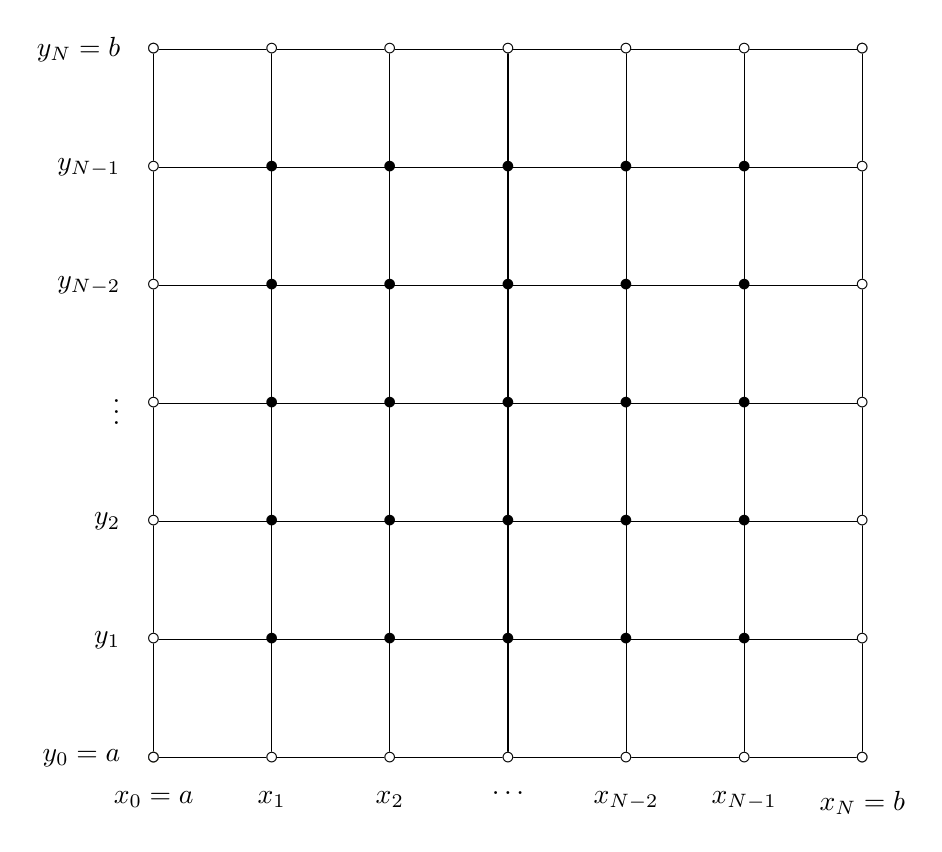
\begin{tikzpicture}[scale=1.5]
	\draw (-3,-3.2) node[below] {$x_0=a$} ;
	\draw (-2,-3.2) node[below] {$x_1$} ;
	\draw (-1,-3.2) node[below] {$x_2$} ;
	\draw (0,-3.2) node[below] {$\ldots$} ;
	\draw (1,-3.2) node[below] {$x_{N-2}$} ;
	\draw (2,-3.2) node[below] {$x_{N-1}$} ;
	\draw (3,-3.2) node[below] {$x_N =b$} ;
	
	\draw (-3.2,-3) node[left] {$y_0=a$} ;
	\draw (-3.2,-2) node[left] {$y_1$} ;
	\draw (-3.2,-1) node[left] {$y_2$} ;
	\draw (-3.2,0) node[left] {$\vdots$} ;
	\draw (-3.2,1) node[left] {$y_{N-2}$} ;
	\draw (-3.2,2) node[left] {$y_{N-1}$} ;
	\draw (-3.2,3) node[left] {$y_N =b$} ;
	
	\draw (-3,-3) grid[step=1] (3,3);

	\draw (-3,-3) node[color=yellow] {$\bullet$} ;
	\draw (-3,-3) node {$\circ$} ;
	
	\foreach \k in {-3,...,3}
		{\draw  (\k,-3) node[color=white] {$\bullet$} ;
	   	\draw (\k,-3) node {$\circ$} ;
	   	\draw  (\k,3) node[color=white] {$\bullet$} ;
	   	\draw (\k,3) node {$\circ$} ;
	   	\draw  (-3,\k) node[color=white] {$\bullet$} ;
	   	\draw (-3,\k) node {$\circ$} ;
	   	\draw  (3,\k) node[color=white] {$\bullet$} ;
	   	\draw (3,\k) node {$\circ$} ;
	   	}
	   	
	\foreach \k in {-2,...,2}
		{\draw  (\k,-2) node {$\bullet$};
		\draw  (\k,-1) node {$\bullet$};
		\draw  (\k,0) node {$\bullet$};
		\draw  (\k,1) node {$\bullet$};
		\draw  (\k,2) node {$\bullet$};
	   	}
\end{tikzpicture}
\end{center}
\caption{Grille en dimension 2. Les symboles $\circ$ désignent les points de bords, les symboles $\bullet$ désignent les points intérieurs de la grille.}
\label{fig:maillage2D}
\end{figure}


On dit qu'une fonction $u : (x,y) \in \mathbb{R} \mapsto u(x,y) \in \mathbb{R}$ est $L-$\textit{périodique} dans les directions $x$ et $y$ si 
\begin{equation}
\begin{array}{rcl}
u(x,y+L) & = & u(x,y) \\
u(x+L,y) & = & u(x,y)
\end{array} \text{ pour tous } (x,y) \in \mathbb{R}^2.
\end{equation}

Comme en dimension 1, nous définissons différentes notions de fonctions discrètes associées à la grille :
\begin{enumerate}
\item Une \textit{fonction de grille} est une fonction définie aux points de la grille $(x_i,y_j)_{0 \leq i,j \leq N}$. Nous notons ces fonctions en fonte gothique comme $\mathfrak{u}$ ou $\mathfrak{v}$. On a :
\begin{equation}
\mathfrak{u} = \left( \mathfrak{u}(x_i,y_j) \right)_{0 \leq i,j \leq N} \text{ et } \mathfrak{u}_{i,j} = \mathfrak{u}(x_i,y_j).
\end{equation}
On note $L^2_h$ l'espace des fonctions de grilles. Cet espace est équipé d'un produit scalaire et de la norme associée :
\begin{equation}
(\mathfrak{u}, \mathfrak{v})_h = h^2 \gsum_{i,j=0}^N \mathfrak{u}(x_i, y_j) \bar{\mathfrak{v}}(x_i, y_j) \text{ et } |\mathfrak{u}|_h = \sqrt{(\mathfrak{u},\mathfrak{u})_h}.
\end{equation}
de plus, on a également
\begin{equation}
| \mathfrak{u} |_{\infty} = \max_{0 \leq i,j \leq N} |\mathfrak{u}(x_i, y_j)|.
\end{equation}
Pour simplifier les notations, nous noterons
\begin{equation}
\mathfrak{u}_{i,j} = \mathfrak{u}(x_i, y_j) \text{ avec } 1 \leq i,j \leq N.
\end{equation}

$\mathfrak{u}$ est périodique si $\mathfrak{u}(x_{i},y_0) = \mathfrak{u}(x_{i},y_N)$ et $\mathfrak{u}(x_{0},y_j) = \mathfrak{u}(x_{N},y_j)$ pour tous $0 \leq i,j \leq N$. On note $L_{h,per}^2$ l'espace des fonctions de grilles périodiques. Cet espace est doté du produit scalaire et de la norme
\begin{equation}
(\mathfrak{u},\mathfrak{v})_{h,per} = h^2 \sum_{i,j=0}^{N-1} \mathfrak{u}_{i,j} \bar{\mathfrak{v}}_{i,j} \text{ et } |\mathfrak{u}|_{h,per} = \sqrt{(\mathfrak{u}, \mathfrak{u})_{h,per}}.
\end{equation}


\item Soit $u : (x,y) \in \Omega \mapsto u(x,y) \in \mathbb{R}$, nous définissons la fonction associée, notée $u^*$ par la restriction de $u$ à la grille :
\begin{equation}
u^*_{i,j} = u(x_i, y_j) \text{ pour tous } 0 \leq i,j \leq N.
\end{equation}

Si $u$ est périodique selon $x$ et $y$, on a $u^*_{i,0}=u^*_{i,N}$ et $u^*_{0,j}=u^*_{N,j}$ pour tous $0 \leq i,j \leq N$.
D'une manière générale, dans un contexte périodique, les données sur des bords opposés du carrés coïncident.





\item A une fonction de grille $\mathfrak{u} \in L^2_h$, on associe un vecteur $U \in \mathbb{R}^{(N+1)^2}$ constitué des valeurs de $\mathfrak{u}$ dans l'ordre anti-lexicographique :
\begin{equation}
U = \begin{bmatrix}
\mathfrak{u}_{0,0}\\
\mathfrak{u}_{1,0}\\
\vdots \\
\mathfrak{u}_{N,0}\\
\mathfrak{u}_{0,1}\\
\mathfrak{u}_{1,1}\\
\vdots \\
\mathfrak{u}_{N,1}\\
\vdots \\
\mathfrak{u}_{N,N}\\
\end{bmatrix}.
\end{equation}
On note ces vecteurs par des lettres capitales.
\end{enumerate}
















\subsection{Opérateurs aux différences en géométrie cartésienne}

En utilisant les notations de la partie \ref{sec:notation_2D} en contexte périodique, nous définissons des opérateurs agissant sur les fonctions de grilles en dimension 2.

\begin{definition}
Soient $\tau_x$ et $\tau_y$ les \textit{opérateurs de translation} dans les directions $x$ et $y$ définis par
\begin{equation}
\left\lbrace
\begin{array}{rcl}
\tau_x \mathfrak{u}_{i,j} & = & \mathfrak{u}_{i+1,j}\\
\tau_y \mathfrak{u}_{i,j} & = & \mathfrak{u}_{i,j+1}\\
\end{array}
\right.
\end{equation}
avec $\mathfrak{u}$ une fonction de grille et $1 \leq i,j \leq N$.
\end{definition}

Les opérateurs obtenus en dimension 1 sont définis en dimension 2 grâce à ces deux opérateurs de translation. On définit les opérateurs centrés dans les directions $x$ et $y$ par 
\begin{equation}
\left\lbrace
\begin{array}{rcl}
\delta_{2P,x} & = & \dfrac{1}{h} Q_{2P}(\tau_x) \\
\delta_{2P,y} & = & \dfrac{1}{h} Q_{2P}(\tau_y)
\end{array}
\right.
\label{eq:der_centrée_2D}
\end{equation}
De la même manière, on définis les opérateurs dans chaque direction par 
\begin{equation}
\left\lbrace
\begin{array}{rcl}
\sigma_x & = & R(\tau_x) \\
\sigma_y & = & R(\tau_y) \\
\end{array}
\right.
\label{eq:simpson_2D}
\end{equation}
Chacun des opérateurs $\sigma_x$ et $\sigma_y$ est inversible si $|\beta|<1/4$.
L'opérateur hermitien en dimension 1 $\delta_x^H$ est étendue en dimension 2 grâce à la relation suivante 
\begin{equation}
\left\lbrace
\begin{array}{rcl}
\delta_{2P,x}^H & = & \sigma_x^{-1} \circ \delta_{2P,x} \\
\delta_{2P,y}^H & = & \sigma_y^{-1} \circ \delta_{2P,y}
\end{array}
\right.
\label{eq:der_herm_2D}
\end{equation}

\begin{theoreme}
Soit $u : x \in \Omega \mapsto u(x) \in \mathbb{R}$ est une fonction de $\mathcal{C}^5 (\Omega)$. On note $u^*$ la fonction de grille associée à $u$ et $u_x^*$ (resp. $u_y^*$) la fonction de grille associée à la dérivée de $u$ dans la direction $x$ (resp. $y$) notée $\partial_x u$ (resp. $\partial_y u$). Alors
\begin{equation}
\begin{array}{rcl}
|u^*_{x} - \delta_{2P,x}^H u^*|_{\infty} &\leq& C h^{2P+2}\\
|u^*_{y} - \delta_{2P,y}^H u^*|_{\infty} &\leq& C h^{2P+2}
\end{array}
\end{equation}
Si les coefficients de $R$ et $Q_{2P}$ vérifient \eqref{eq:hermitian_system}.
\end{theoreme}

\begin{proof}
Conséquence du théorème \ref{th:consistence_herm2} appliqué dans chaque direction $x$ et $y$.
\end{proof}

























\subsection{Écriture matricielle des opérateurs aux différences en dimension 2}

Dans cette section, nous précisons les notations vectorielles et matricielles utiles à l'écriture matricielle des opérateurs en dimension 2.

Nous définissons la \textit{base canonique} de $\mathbb{R}^N$, notée $\left(e_i \right)_{0 \leq i \leq N-1}$ et donnée par 
\begin{equation}
\left( e_i \right) = \delta_{i,j} = \left\lbrace
\begin{array}{rl}
1 & \text{ si } j=i,\\
0 & \text{ sinon.}
\end{array}
\right.
\end{equation}
$\delta_{i,j}$ est le symbole de Kronecker.

\begin{definition}
Soit $A$ une matrice de taille $m \times n$ et $B$ une matrice de $p \times q$, avec $m, n, p, q \in \mathbb{N}^{\star}$. La matrice $A \otimes B$ est une matrice de taille $mp \times nq$ donnée comme le produit de Kronecker de $A$ par $B$ et 
\begin{equation}
A \otimes B = 
\begin{bmatrix}
a_{1,1}B & \cdots & a_{1,n}B \\ 
\vdots & \ddots & \vdots \\ 
a_{n,1}B & \cdots & a_{n,n}B
\end{bmatrix} 
\end{equation}
\end{definition}
On rapelle les propriétés suivantes concernant le produit de Kronecker :

\begin{proposition}
Soient $A$, $B$, $C$ et $D$ des matrices et $\alpha$ un réel.
\begin{itemize}
\item La multiplication par un scalaire vérifie
\begin{equation}
\alpha ( A \otimes B ) = \alpha A \otimes B = A \otimes \alpha B,
\end{equation}

\item si les produits $AC$ et $BD$ sont bien définis alors
\begin{equation}
(A \otimes B ) (C \otimes D) = AC \otimes BD,
\end{equation} 


\item si $A$ et $B$ sont inversibles
\begin{equation}
(A \otimes B)^{-1} = A^{-1} \otimes B^{-1}.
\end{equation}
\end{itemize}
\label{prop:pdt_kron}
\end{proposition}
L'application $\text{vec}_2$ permet de transformer une fonction de grille $\mathbf{u}$ en un vecteur $U$.

\begin{definition}
L'opérateur $\text{vec}_2$ est défini par
\begin{equation}
\begin{array}{rcl}
\text{vec}_2 : L^2_h & \longrightarrow & \mathbb{R}^{N^2}\\
\mathfrak{v} & \longrightarrow & V = \text{vec}_2(\mathfrak{v})
\end{array}
\end{equation}
avec
\begin{equation}
\text{vec}_2(\mathfrak{v}) = \gsum_{i,j=0}^{N-1} \left( e_j \otimes e_i \right)\mathfrak{v}_{i,j}.
\end{equation}
\end{definition}

L'opérateur $\text{vec}_2$ transforme une fonction de grille $\mathfrak{v}$ en un vecteur en organisant les données dans l'ordre antilexicographique. Si $V = \text{vec}_2 (\mathfrak{v})$ alors on a l'égalité suivante :
\begin{equation}
V=[\mathfrak{v}_{1,1}, \mathfrak{v}_{2,1}, \mathfrak{v}_{3,1}, \cdots, \mathfrak{v}_{N,1}, \mathfrak{v}_{1,2}, \mathfrak{v}_{2,2}, \cdots,  \mathfrak{v}_{N-1,N}, \mathfrak{v}_{N,N}]^T
\end{equation}

\begin{proposition}
Soit $\mathfrak{u}$ une fonction de grille. Alors les opérateurs de dérivées centrées \eqref{eq:der_centrée_2D} s'écrivent matriciellement sous la forme
\begin{equation}
\left\lbrace
\begin{array}{rcl}
\text{vec}_2(\delta_{2P,x} \mathfrak{u}) & = & (Id \otimes D_{2P}) \text{vec}_2(\mathfrak{u})\\
\text{vec}_2(\delta_{2P,y} \mathfrak{u}) & = & (D_{2P} \otimes Id) \text{vec}_2(\mathfrak{u})\\
\text{vec}_2(\sigma_x \mathfrak{u}) & = & (Id \otimes P) \text{vec}_2(\mathfrak{u})\\
\text{vec}_2(\sigma_y \mathfrak{u}) & = & (P \otimes Id) \text{vec}_2(\mathfrak{u})\\
\end{array}\right.
\end{equation}
\label{prop:op_der_simpson_mat}
\end{proposition}

\begin{proof}
Par définition de $\text{vec}_2$, on a 
\begin{align*}
\text{vec}_2 (\delta_{2P,x} \mathfrak{u}) & = \gsum_{i,j=0}^P (e_j \otimes e_i) \delta_{2P,x} \mathfrak{u}_{i,j} \\
	& = \gsum_{i,j=0}^{N-1} \gsum_{p=1}^P (e_j \otimes e_i) \dfrac{a_p}{2ph} (\mathfrak{u}_{i+p,j} - \mathfrak{u}_{i-p,j}) \\
	& = \gsum_{p=1}^P \dfrac{a_p}{2ph} \left( \gsum_{i,j=0}^{N-1} (e_j \otimes e_i) \mathfrak{u}_{i+p,j} - (e_j \otimes e_i) \mathfrak{u}_{i-p,j} \right) \\
	& = \gsum_{p=1}^P \dfrac{a_p}{2ph} \gsum_{i,j=0}^{N-1} e_j \otimes \left( e_j \otimes (e_i \mathfrak{u}_{i+p,j} - e_i \otimes \mathfrak{u}_{i-p,j}) \right)\\
	& = \gsum_{p=1}^P \dfrac{a_p}{2ph} \left( Id \otimes \left( T^p - T^{-p}  \right) \right) \vec_2 (\mathfrak{u}) \\
	& = (Id \otimes D_{2P}) \vec_2 (\mathfrak{u})
\end{align*}
les autres égalités se montrent de la même manière
\end{proof}

De ces égalités, il découle le calcul matriciel de $\delta_{2P,x}^H \mathfrak{u}$ et de $\delta_{2P,y}^H \mathfrak{u}$.

\begin{theoreme}
Soit $\mathfrak{u}$ une fonction de grille. Alors, si on pose 
\begin{equation}
\left\lbrace
\begin{array}{rcl}
U & = & \text{vec}_2 (\mathfrak{u}) \\
U_x & = & \text{vec}_2 (\delta_{2P,x}^H \mathfrak{u}) \\
U_y & = & \text{vec}_2 (\delta_{2P,y}^H \mathfrak{u}) \\
\end{array}
\right.
\end{equation}
alors les égalités suivantes sont vérifiées
\begin{equation}
\left\lbrace
\begin{array}{rcccl}
U_x &=& (Id \otimes P)^{-1}(Id \otimes D_{2P}) U &=& (Id \otimes P^{-1}D_{2P})U \\
U_y &=& (P \otimes Id)^{-1}(D_{2P} \otimes Id) U &=& (P^{-1}D_{2P} \otimes Id)U\\
\end{array}
\right.
\end{equation}
\end{theoreme}

\begin{proof}
Conséquence directe des propositions \ref{prop:op_der_simpson_mat} et \ref{prop:pdt_kron}.
\end{proof}

La matrice du schéma hermitien $(Id \otimes P^{-1}K)$ en direction $x$ et $(P^{-1}K \otimes Id)$ en direction $y$ vérifient des propriétés d'antisymétriques similaires à celles en dimension 1.
\begin{proposition}
Les matrices $(Id \otimes P^{-1}K)$ et $(P^{-1}K \otimes Id)$ sont antisymétrique.
\end{proposition}

\begin{proof}
$P^{-1}K$ est antisymétrique. D'où le résultat.
\end{proof}








\subsection{Opérateur de filtrage}

Dans cette partie, nous utilisons toujours les notations de la section \ref{sec:notation_2D} en contexte périodique. Définissons les opérateurs de filtrage dans les directions $x$ et $y$ par
\begin{eqnarray*}
\mathcal{F}_x = \gsum_{k=0}^F a_k \dfrac{\tau_x^k + \tau_x^{-k}}{2}  = S(\tau_x)\\
\mathcal{F}_y = \gsum_{k=0}^F a_k \dfrac{\tau_y^k + \tau_y^{-k}}{2} = S(\tau_y) \\
\end{eqnarray*}

Avec $(a_k)_{0 \leq k \leq F}$ vérifiant le système \eqref{prop:filter_def}. Comme la géométrie est cartésienne, on remarque que 
\begin{equation}
\mathcal{F}_x \circ \mathcal{F}_y = \mathcal{F}_y \circ \mathcal{F}_x.
\end{equation}
Ce qui est faux lorsque la métrique n'est pas orthogonale.
La proposition \ref{prop:filter_def} permet de vérifier la consistance des opérateurs de filtrages.
Si $u : (x,y) \in \Omega \mapsto u(x,y) \in \mathbb{R}$ est fonction de $\mathcal{C}^{2F}$ alors :
\begin{eqnarray*}
\mathcal{F}_x u^*_{i,j} - u^*_{i,j} & = & C_xh^{2F}\\
\mathcal{F}_y u^*_{i,j} - u^*_{i,j} & = & C_yh^{2F}
\end{eqnarray*}
où $C_x$ et $C_y$ sont des constantes indépendantes de $h$.
En particulier, en composant les opérateurs, on peut définir un nouvel opérateur de filtrage. En effet  
\begin{equation}
(\mathcal{F}_x \circ \mathcal{F}_y) u_{i,j}^* - u_{i,j}^* = Ch^{2F}.
\end{equation}

L'écriture matricielle de l'opérateur de filtrage est donnée par la proposition suivante :
\begin{proposition}
Soit $\mathbf{u}$ une fonction de grille. Alors les opérateurs de filtrages s'écrivent à l'aide de matrices comme :
\begin{equation}
\left\lbrace
\begin{array}{rcl}
\text{vec}_2 (\mathcal{F}_x \mathbf{u}) & = & (Id \otimes M) \text{vec}_2 (\mathbf{u})\\
\text{vec}_2 (\mathcal{F}_y \mathbf{u}) & = & (M \otimes Id) \text{vec}_2 (\mathbf{u})\\
\end{array}
\right.
\end{equation}
\end{proposition}
Comme la matrice $M$ est symétrique, il est immédiat que $Id \otimes M$ et $M \otimes Id$ sont symétriques aussi.